\documentclass[journal=esthag,manuscript=article]{achemso}

% additional packages
\usepackage[utf8]{inputenc}
\usepackage{amsmath}
\usepackage{booktabs}
\usepackage{subcaption}
\usepackage{tabularx}
\usepackage{array,multirow,graphicx}
\usepackage{comment}
\graphicspath{
  {./../figures/},
  {./../figures/air-exchange-rate/},
  {./../figures/kde-iacc-pressure/},
  {./../figures/preferential-pathway-sensitivity/},
  {./../figures/transient-response/}
}
\usepackage{lineno}
\linenumbers
% macros

% authors
\author{Jonathan G. V. Ström}
\affiliation[Brown University]{Brown University, School of Engineering, Providence, RI, USA}
\author{Yijun Yao}
\affiliation[Zhejiang University]{Zhejiang University, Hangzhou, China}
\author{Eric M. Suuberg}
\email{eric_suuberg@brown.edu}
\affiliation[Brown University]{Brown University, School of Engineering, Providence, RI, USA}

% title
\title{Transient Variability In Vapor Intrusion And The Factors That Influence It}

% keywords
\abbreviations{VI}
\keywords{VI, Preferential pathways, Temporal transient variability}

\begin{document}

\begin{abstract}
Temporal variability in indoor air contaminant concentrations at vapor intrusion (VI) sites has been a concern for some time.
We consider the source of the variability at VI sites located near Hill Air Force Base and Naval Air Station North Island using statistical analysis methods and three-dimensional subsurface computational fluid dynamics modeling.
The results suggest that an order of magnitude variation in indoor air contaminant concentrations may be expected at ”normal” VI sites where preferential pathways do not play a role, whereas three or more orders of magnitude can be observed at sites characterized by preferential pathways.
A CFD modeling sensitivity analysis reveals that it is not only the presence of contaminant vapor in a preferential pathway that is required to see large observed variations, but there must also exist a permeable region beneath the structure.
Large temporal fluctuations in indoor air contaminant concentrations may be observed where no preferential pathways exist, but this requires a particular combination of large fluctuations in pressure driving force and high soil permeability.
\end{abstract}

\section{Introduction}

Long term vapor intrusion (VI) studies in both residential and larger commercial structures have raised concerns regarding significant observed transient behavior in indoor air contaminant concentrations\cite{u.s._environmental_protection_agency_oswer_2015,folkes_observed_2009,holton_temporal_2013,johnston_spatiotemporal_2014,hosangadi_high-frequency_2017,mchugh_recent_2017}.
VI involves the migration of volatilizing contaminants from soil, groundwater or other subsurface sources into overlying structures. VI has been a recognized problem for some time, but many aspects remain poorly understood, particularly with respect to the causes of large temporal transients in indoor air concentrations.
There is uncertainty within the VI community regarding how to best develop sampling strategies to address this problem\cite{u.s._environmental_protection_agency_oswer_2015,holton_temporal_2013,johnson_integrated_2016}. \par

Results from a house operated by Arizona State University (ASU) near Hill AFB in Utah, an EPA experimental house in Indianapolis, IN and a large warehouse at the Naval Air Station (NAS) North Island, CA have all shown significant transient variations in indoor air contaminant concentrations.
All were outfitted with sampling and monitoring equipment that allowed tracking temporal variation in indoor air contaminant concentrations on time scales of hours.
All have shown that these concentrations varied significantly with time - orders of magnitude on the timescale of a day or days.
\cite{holton_evaluation_2015,guo_vapor_2015,hosangadi_high-frequency_2017}. \par

In one instance the source of the variation was clearly established during the study; at the ASU house a field drain pipe (or “land drain”), which connected to a sewer system, was discovered beneath the house, and careful isolation of this source led to a clear conclusion that this preferential pathway significantly contributed to observed indoor air contaminant levels and their fluctuations\cite{guo_vapor_2015,guo_identification_2015}.
While in this case the issue of a contribution from a preferential pathway was clearly resolved, what it left open was a question of whether existence of such a preferential pathway to an area beneath a structure would always be expected to lead to large fluctuations in indoor air contaminant concentrations. \par

Similarly, a sewer pipe has recently been suggested to be a source of the contaminants found in the EPA Indianapolis house\cite{mchugh_evidence_2017}.
That site was also characterized by large indoor air contaminant concentration fluctuations.
Sewer lines have been generally implicated as VI source at several sites to date\cite{pennell_sewer_2013,mchugh_evidence_2017,roghani_occurrence_2018,riis_vapor_2010}.
A Danish study estimates that roughly 20\% of all VI sites in central Denmark involve significant sewer VI pathways\cite{nielsen_remediation_2017}.
Thus while the consideration of a role of possible sewer or other preferential pathways is now part of normal good practice in VI site investigation, it is still not known whether the existence of such pathways automatically means that large temporal fluctuations are necessarily to be expected.
In some of these cases\cite{pennell_sewer_2013,riis_vapor_2010}, the sewer provided a pathway for direct entry of contaminant into the living space.
While potentially important in many cases, this scenario is not further considered here, where the focus is on pathways that deliver contaminant to the soil beneath a structure. \par

It is, however, now known that even absent a preferential pathway, there may be significant transient variation in indoor air contaminant concentrations at VI sites\cite{folkes_observed_2009,brenner_results_2010,johnston_spatiotemporal_2014}.
One example is a site at NAS North Island at which no preferential pathways have been identified.
Instead, a building at this site is characterized by significant variations in indoor-outdoor pressure differential\cite{hosangadi_high-frequency_2017}.
It is believed that this is the origin of the fluctuations at that site. \par

This paper investigates the sources of the temporal variation in indoor air contaminant concentrations in both the presence and absence of in soil preferential pathways.
In this work, the latter scenarios are referred to as ”normal” VI scenarios, in which there is typically a groundwater source of the contaminant.
Specifically, we pose the question of just how much variation in indoor air contaminant concentration may be expected at  such normal  VI  sites vs. those characterized by preferential pathways.
The conditions required for preferential pathways to be significant contributors to temporal variations in indoor air contaminant concentrations are also explored, and the consequences for sampling strategies are also discussed.

\section{Methods}

\subsection{Statistical Analysis Of Field Data}

To begin to characterize transient behavior in indoor air contaminant concentrations, actual datasets are analyzed to establish common levels of variability at VI sites.
For this purpose, the datasets from the ASU house in Utah, the EPA Indianapolis site and North Island NAS were chosen for analysis.
This paper relies on statistical analysis of published field data, and readers are referred to the original works for details regarding data acquisition\cite{holton_evaluation_2015,guo_vapor_2015,holton_temporal_2013,hosangadi_high-frequency_2017,u.s._environmental_protection_agency_assessment_2015}. \par

The ASU house and data were obtained over a period of a few years.
During part of this time, controlled pressure method (CPM) tests were being conducted, in which the house was underpressurized to an extent greater than that characterizing “normal” operation.
This caused greater than normal advective flow from the subsurface into the house, thus increasing VI potential\cite{mchugh_evaluation_2012,mchugh_recent_2017,holton_evaluation_2015}.
This period of CPM testing is considered separately from the otherwise ”natural” VI conditions in the analysis.
Likewise, the existence of a preferential pathway at the ASU house needs to be considered in examining the dataset, noting that during some of the testing, this pathway was deliberately cut off, resulting in what we have termed “normal” VI conditions in which the main source of contaminant was believed to be groundwater. \par

The NAS North Island dataset has not (as far as is known) been influenced by a preferential pathway, but the structure there was subject to large internal pressure fluctuations, much more extensive than those typically recorded at the ASU house during normal operations.
Additionally, the underlying soil at NAS North Island is sandy and more permeable than that at the ASU site, which, as will be shown, contributes to the indoor air contaminant concentrations being more sensitive to pressure fluctuations\cite{hosangadi_high-frequency_2017}. \par

Likewise, the Indianapolis site investigation spanned over a number of years and periodically included the testing of a sub-slab depressurziation system (SSD).
The goal of which is to mitigate the VI risk by drastically depressurizing the sub-slab area underneath the house, preventing the contaminants from entering the structure above, and therefore only the period before the installation of this system was considered in the analysis.
It is likely a sewer line beneath the structure acted as a preferential pathway\cite{mchugh_evidence_2017}, however at no point was this PP removed, making it difficult to assess how significant the PP was at this site, regardless it is of interest to analyze this site due to its wealth of data. \par

The typical variation in indoor air contaminant concentrations with time will first be considered below in the case of the ASU house during ”natural”, (i.e. non-CPM conditions), in the case of the NAS North Island site over the entire available dataset, and for the Indianapolis case we consider the variations before the installation of the SSD system.
The deviations from the mean TCE (Chloroform and PCE at the Indianapolis site) in indoor air concentration, as well as the indoor-outdoor pressure differential associated with these concentration fluctuations, were examined, and both univariate and bivariate kernel density estimations (KDE) were constructed.
KDE is a technique that estimates the probability distribution of a random variable(s) by using multiple kernels, or weighting functions, and in this case, Gaussian kernels are used to create the KDEs.
This means that it is presumed that the variables of interest (i.e., indoor air contaminant concentrations and indoor-outdoor pressure differentials, as sampled) are normally distributed around mean values (that there is statistical fluctuation associated with each sampling event).
In this instance, the scipy statistical package was used to construct the KDEs, assuming a bandwidth parameter determined by Scott's rule.
The distributions of the individual parameters and the relationship between them will be examined using the KDE method.

\subsection{Modeling Work}
In addition to examining the actual field data, a previously described three -dimensional computational fluid dynamics model of a generic VI impacted house was used to elucidate certain aspects of  the processes.
This model was implemented in a finite element solver, COMSOL Multiphysics.
In the present work, there has been an addition of a preferential pathway to the ”standard” model that has been described before in publications by this group\cite{shen_influence_2013,yao_investigating_2017,yao_three-dimensional_2017}.
In this modeling work, only the vadose zone soil domain is directly modeled.

The modeled structure is assumed to have a 10x10 m foundation footprint, with the bottom of the foundation slab lying 1 m below ground surface (bgs), simulating a house with a basement.
The indoor air space is modeled as a continuously stirred tank (CST)\cite{u.s._environmental_protection_agency_oswer_2015} and all of the contaminant entering the house is assumed to enter with soil gas through a 1 cm wide crack located between the foundation walls and the foundation slab that spans the perimeter of the house.
All of the contaminant leaving the indoor air space is assumed does so via air exchange with the ambient.
The indoor control volume is assumed to consist of only of the basement, assumed as having a total volume of $300 \; \mathrm{m^3}$.
Clearly different assumptions could be made regarding the structural features and the size of the crack entry route, but for present purposes, this is unimportant as the intent is only to show for “typical” values what the influence of certain other features can be.
The modeled surrounding soil domain extends 5 meters from the perimeter of the house, and is assumed to consist of sandy clay (except as noted).
Directly beneath the foundation slab, there is assumed to be a 30 cm (one foot) thick gravel layer, except in certain cases where this sub-base material is assumed to be the same as the surrounding soil (termed  a ”uniform” soil scenario).
The preferential pathway is modeled as a 10 cm (4”) pipe that exits into the gravel sub-base beneath the structure.
The air in the pipe is assumed to be contaminated with TCE at a vapor concentration equal to the vapor in equilibrium with the groundwater contaminant concentration below the structure, modified by a scaling factor $\chi$, which is allows the contaminant concentration in the pipe to be parameterized.
The groundwater beneath the structure is assumed to be homogeneously contaminated with trichloroethylene (TCE) as a prototypical contaminant.
The groundwater itself is not modeled, as the bottom of the model domain is defined by the top of the water table.
The ground surface and the pipe are both assumed to be sources of air to the soil domain.
Both are assumed to be at reference atmospheric pressure.
Vapor transport in the soil is governed by Richard’s equation, a modified version  of Darcy’s Law, taking the variability of soil moisture in the vadose zone into account\cite{richards_capillary_1931}.
The van Genuchten equations are used to predict the soil moisture content and thus the effective permeability of the soil\cite{van_genuchten_closed-form_1980}.
The effective diffusivity of contaminant in soil is calculated using the Millington-Quirk model\cite{millington_permeability_1961}.
The transport of vapor contaminant in the soil is assumed to be governed by the advection-diffusion equation, in which either advection or diffusion may dominate depending upon position and particular circumstances.
The equations and the boundary conditions are given in Table \ref{tbl:eqns-bc-parameters}.

\begin{table}[htb!]
  \centering
  \caption{Governing equations, boundary conditions \& model input parameters. (See below for table of nomenclature).}
  \label{tbl:eqns-bc-parameters}
  \bigskip
  %%%%%%%%%%%%%%%%%%%%%%%%%%%%%%%%%%%%%%%%%%%%%%%%%%%%%%%%%%%%%%%%%%%%%%%%%%%%%%
  % Governing equations
  %%%%%%%%%%%%%%%%%%%%%%%%%%%%%%%%%%%%%%%%%%%%%%%%%%%%%%%%%%%%%%%%%%%%%%%%%%%%%%
  \subcaption{Governing equations}
  \begin{tabular}{l l}
    \toprule
    % Indoor air space equation
    Unsteady-CSTR                 & $V\frac{d u}{d t} = \int_{A_\mathrm{ck}} j_\mathrm{ck} dA - u A_e V$ \\
    % Richard's equation
    Richard's equation            & $\nabla \cdot \rho \Big( - \frac{\kappa_s}{\mu} k_r \nabla p \Big) = 0$ \\
    % Millington-Quirk equation
    Millington-Quirk              & $D_\mathrm{eff} = D_\mathrm{air}\frac{\theta_g^{10/3}}{\theta_t^2} + \frac{D_\mathrm{water}}{K_H} \frac{\theta_w^{10/3}}{\theta_t^2}$ \\
    % Advection-diffusion equation
    Advection-diffusion equation  & $\frac{\partial}{\partial t} \Big( \theta_w c_w + \theta_g c \Big) = \nabla (D_\mathrm{eff} \cdot \nabla c) - \vec{u} \cdot \nabla c$ \\
    % van Genuchten's equations
    \multirow{3}{*}{van Genuchten equations}     & $\mathrm{Se} = \frac{\theta_w - \theta_r}{\theta_t - \theta_r} = [1 + |\alpha z|^n]^{-m}$ \\
                                  & $\theta_g = \theta_t - \theta_w$ \\
                                  & $k_r = (1 - \mathrm{Se})^{l} [1 - (\mathrm{Se}^{-m})^m]^2$ \\
                                  & $m = 1 - 1/n$ \\
    \bottomrule
  \end{tabular}
  \bigskip
  %%%%%%%%%%%%%%%%%%%%%%%%%%%%%%%%%%%%%%%%%%%%%%%%%%%%%%%%%%%%%%%%%%%%%%%%%%%%%%
  % Boundary conditions
  %%%%%%%%%%%%%%%%%%%%%%%%%%%%%%%%%%%%%%%%%%%%%%%%%%%%%%%%%%%%%%%%%%%%%%%%%%%%%%
  \subcaption{Boundary conditions}
  \begin{tabular}{l l l}
    \toprule
    \textbf{Boundary}          & \textbf{Richard's equation}      &   \textbf{Advection-diffusion equation} \\
    % Foundation crack
    At foundation crack  & $p = p_\mathrm{in/out} \; \mathrm{(Pa)}$                            & $j_\mathrm{ck} = \frac{u c}{1 - \exp{(u L_\mathrm{slab}/D_\mathrm{air})}}$ \\
    % Groundwater source
    At groundwater source &  N/A & $c = c_\mathrm{gw} K_H \; \mathrm{(\mu g/m^3)}$ \\
    % Ground surface
    At ground surface      & $p = 0 \; \mathrm{(Pa)}$  & $c = 0 \; \mathrm{(\mu g/m^3)}$ \\
    % Preferential pathway
    Exit of preferential pathway  & $p = 0 \; \mathrm{(Pa)}$  & $c = c_\mathrm{gw} K_H \chi \; \mathrm{(\mu g/m^3)}$ \\
    \bottomrule
  \end{tabular}
  \bigskip
  %%%%%%%%%%%%%%%%%%%%%%%%%%%%%%%%%%%%%%%%%%%%%%%%%%%%%%%%%%%%%%%%%%%%%%%%%%%%%%
  % Soil input parameters
  %%%%%%%%%%%%%%%%%%%%%%%%%%%%%%%%%%%%%%%%%%%%%%%%%%%%%%%%%%%%%%%%%%%%%%%%%%%%%%
  \subcaption{Soil \& gravel properties\cite{dan_capillary_2012,abreu_conceptual_2012,u.s._environmental_protection_agency_userss_2004}}
  \begin{tabular}{l l l l l l l}
    \toprule
    % Descriptions
    Soil & $\text{Permeability} \; \mathrm{(m^2)}$  & $\mathrm{Density} \; \mathrm{(kg/m^3)}$  & $\theta_s$  & $\theta_r$  & $\alpha \; \mathrm{(1/m)}$  & $n$ \\
    % Gravel
    Gravel     & $1.3 \cdot 10^{-9}$   & 1680    & 0.42        & 0.005       & 100       & 3.1 \\
    % Sand
    Sand     & $9.9 \cdot 10^{-12}$  & 1430    & 0.38        & 0.053        & 3.5       & 3.2 \\
    % Sandy clay
    Sandy Clay    & $1.7 \cdot 10^{-14}$  & 1470    & 0.39        & 0.12        & 3.3       & 1.2 \\
    \bottomrule
  \end{tabular}
  \bigskip
  %%%%%%%%%%%%%%%%%%%%%%%%%%%%%%%%%%%%%%%%%%%%%%%%%%%%%%%%%%%%%%%%%%%%%%%%%%%%%%
  % TCE input parameters
  %%%%%%%%%%%%%%%%%%%%%%%%%%%%%%%%%%%%%%%%%%%%%%%%%%%%%%%%%%%%%%%%%%%%%%%%%%%%%%
  \subcaption{Trichloroethylene (diluted in air) properties\cite{abreu_conceptual_2012,u.s._environmental_protection_agency_userss_2004}}
  \begin{tabular}{l l l l l l}
    \toprule
    $D_\mathrm{air} \; \mathrm{(m^2/h)}$  & $D_\mathrm{water} \; \mathrm{(m^2/h)}$  & $\mathrm{Density} \; \mathrm{(kg/m^3)}$ & $\mathrm{Viscosity} \; \mathrm{(Pa \cdot s)}$  & $K_H$ & $M \; \mathrm{(g/mol)}$ \\
    $2.47 \cdot 10^{-2}$  & $3.67 \cdot 10^{-6}$  & 1.614 & $1.86 \cdot 10^{-5}$  & 0.403 & 131.39 \\
    \bottomrule
  \end{tabular}
  \bigskip
  %%%%%%%%%%%%%%%%%%%%%%%%%%%%%%%%%%%%%%%%%%%%%%%%%%%%%%%%%%%%%%%%%%%%%%%%%%%%%%
  % Building input parameters
  %%%%%%%%%%%%%%%%%%%%%%%%%%%%%%%%%%%%%%%%%%%%%%%%%%%%%%%%%%%%%%%%%%%%%%%%%%%%%%
  \subcaption{Building properties}
  \begin{tabular}{l l l}
    \toprule
    $V_\mathrm{base} \; \mathrm{(m^3)}$  & $L_\mathrm{slab} \; \mathrm{(cm)}$  & $A_e \; \mathrm{(1/hr)}$ \\
    %
    300  &  15  & 0.5 \\
    \bottomrule
  \end{tabular}
\end{table}

\subsection{Drivers For Indoor Air Contaminant Variability}
\subsubsection{The Role Of Building Depressurization/Pressurization}
% KDE figures
\begin{figure}[htb!]
  \caption{KDE analysis of IACC dependence on indoor/outdoor pressure difference at the ASU house and North Island site (\ref{fig:kde-asu-nas}) and the Indianapolis site (\ref{fig:kde-indianapolis}). p-values and Pearson's r-values shown for each dataset.}
  \label{fig:kde-analysis}
  % ASU/North Island plot
  \begin{subfigure}{\textwidth}
    \centering
    \caption{Period before and after the PP was shut at the ASU house considered separately; North Island dataset considered in its entirety.}
    \label{fig:kde-asu-nas}
    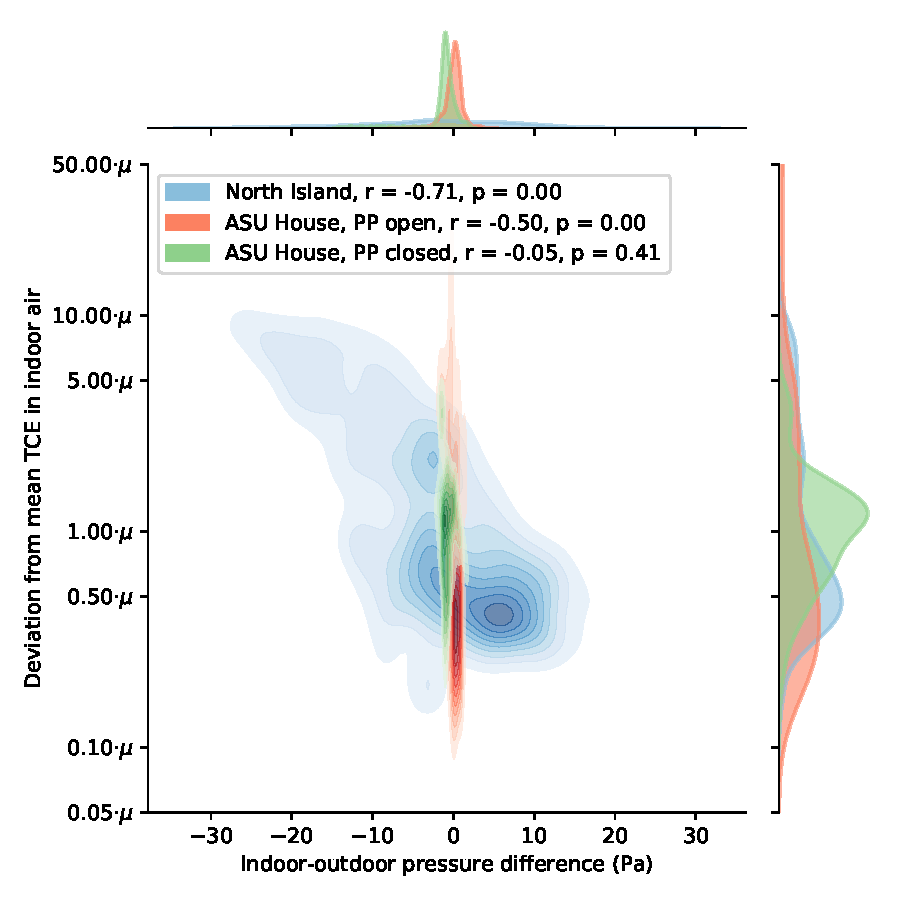
\includegraphics[height=0.4\textheight,keepaspectratio]{nas-asu-house-iacc-deviating.pdf}
  \end{subfigure}
  % Indianapolis plot
  \begin{subfigure}{\textwidth}
    \centering
    \caption{Chloroform and PCE considered separeately at Indianapolis duplex 422.}
    \label{fig:kde-indianapolis}
    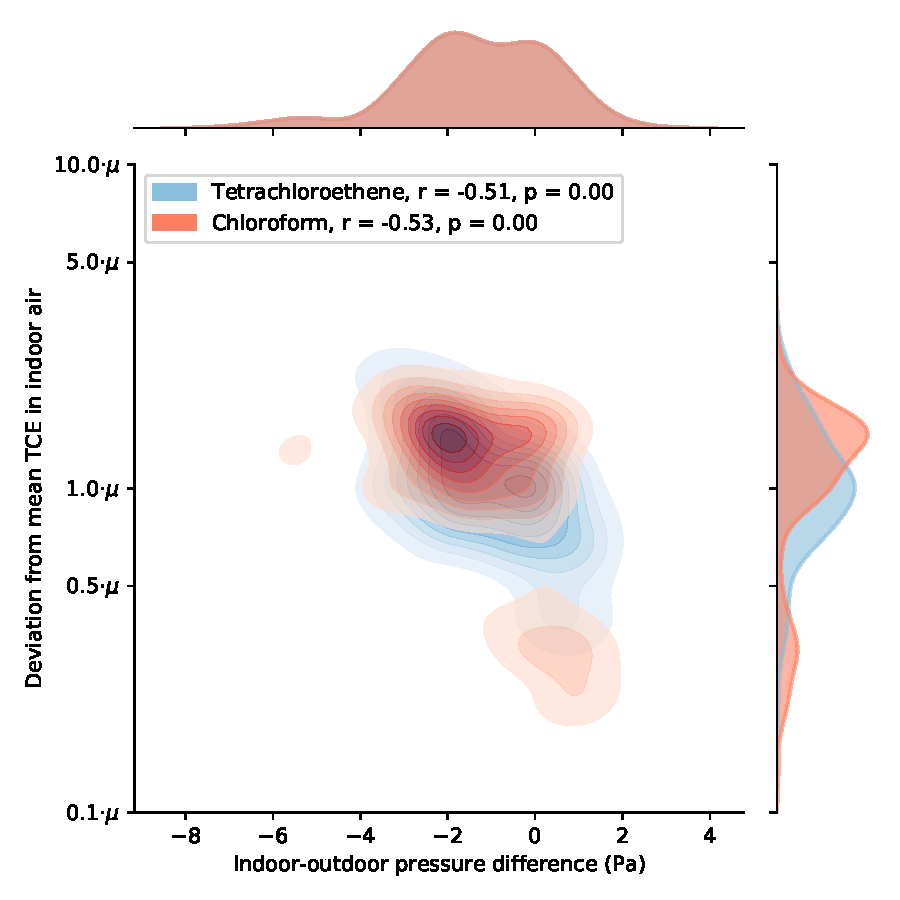
\includegraphics[height=0.4\textheight,keepaspectratio]{indianapolis-422.pdf}
  \end{subfigure}
\end{figure}
% Introduction
Out of the factors that influence IACC in VI, pressure is one of the most dynamic ones, and the relationship between changes in indoor/outdoor pressure difference and IACC are examined in Figure \ref{fig:kde-analysis}.
Three well-studied VI sites are considered, the "ASU house" near Hill AFB in Utah, a building at North Island NAS in California and a duplex in Indianapolis.\par
% Univariate IACC description
The absolute IACC at these sites vary significantly, therefore some means of comparing them all to each other is necessary.
Additionally, the focus in this section is the driver for variations in IACC, and representation of the variations between the different sites must also be achieved, specifically variations on the scale of order of magnitudes is of the greatest interest, as these are the largest hinderance to proper site IACC characterization.
To achieve these goals, the log-10 deviation from the mean IACC ($\mu$) within each dataset is calculated, e.g. $10\mu$ indicates the IACC is an order of magnitude above the mean IACC for the dataset.
On the y-margin in figures \ref{fig:kde-asu-nas} and \ref{fig:kde-indianapolis}, the univariate KDE distribution of deviation from the mean may be seen. \par
% Univariate pressure description
The indoor/outdoor pressure differences are simply taken as it, and their univariate KDE distributions are shown on the x-margin.
A negative pressure difference indicate that the building is underpressurized relative to outdoor.\par
% Bivariate description
The relationship between the deviation from mean IACC, and indoor/outdoor pressure difference may be seen in the central portion of each figure, in the form of a bivariate KDE distribution.
The p-value and Pearson's r-value for each bivariate distribution is shown in the legend.\par
% Sub-figure description (details about sites)
In Figure \ref{fig:kde-asu-nas} the North Island and ASU house datasets are plotted, with blue representing the North Island site, and with red and green representing the ASU house.
The ASU house dataset is split into two different parts, the first (red) is data from the time period before the PP was discovered, the second (green) is from after the PP was sealed off.
At both of these sites, TCE was the only contaminant considered.
The IACC of Chloroform and PCE in the 422 part of the Indianapolis duplex are considered in Figure \ref{fig:kde-indianapolis}.\par
% North Island discussion
From Figure \ref{fig:kde-asu-nas}, it is apparent that the three datasets differ significantly from each other.
The North Island site exhibit the greatest variation in both pressure difference and IACC, in fact, looking at the univariate pressure distribution - it is almost entirely flat and spanning from extremly high and low values.
A likely explation for this is the poor condition of the structure, rendering it highly susceptible to envivornmental influnces.\par

To accompany this, there is significant variation in IACC, that has a relativly strong link with pressure difference ($r = -0.71$), although there is clearly a distinct peak (around $0.5\mu$) that is primally associated with the smaller negative and positive pressure differences ($~-4 \leq \Delta p \leq 8$).
This demonstrates that at this particular site, the very large variations (an order of magnitude or more) are primarily influenced by the unusually large pressure difference fluctations.
Likely, this relationship is amplified by the fact that the soil surrounding the structure is sandy and therefore relatively permeable - increasing the influence of pressure differences.
However, despite all this, pressure differences can only partly explain the variations observed at this site.\par
% ASU discussion
The two ASU datasets are not only significantly different from the North Island dataset, but also different from each other.
Consider the dataset before the PP was discovered (red) and one can see that the IACC varies significantly (from $0.05 \mu$ to more than $50 \mu$, albeit rarely.)
This is more variation than was observed at North Island, and yet the distribution of pressure differences is narrow, mostly varying by a few Pa around zero (~$\pm 2$ Pa), and with $r = -0.50$, suggests that pressure difference is not insignificant but still a weak predictor for the variations in IACC.\par

The picture changes completely after the PP was closed off, where a similar distribution of pressure differences is observed, but with a signficant reduction in IACC variance to around $\pm 0.5 \mu$, resembling something of a log-normal distribution.
This clearly shows just how much variance the PP at this site contributed with, and how critical it is to assess whether a PP is present at a particular site in general, lest potentially face unacceptable uncertainty in determining the relevant contaminant exposure.
It is also clear that in the absence of a PP, the pressure difference becomes even less important, with the p- and r-value indicating that pressure differences are here insignficant in determining variation in IACC.
This also suggests that the PP at the ASU house acted not only as a PP for contaminant vapors, but for air in general - allowing the impermeable soil surrounding the house to be circumvented.
PPs, and the factors that influnce them will be explored later in this article.\par
% Indianapolis discussion
The Indianapolis duplex also featured a PP, but despite this, there is significantly less variance in IACC of both Chloroform and PCE.
The exact reason for this is not known, but considering that the PP at the Indianapolis site was a sanitary sewer, and at ASU the PP was a foundation drain system, it is not inconceivable that their dynamics are quite different.
Nevertheless, both PCE and Chloroform are more or less log-normally distributed, with (mostly) less than an order of magnitude variance around the mean, indicating that the varation in IACC are species independent.\par

The pressure difference distribution exhibit some bimodal characteristics, with a larger variation than was observed at the ASU site.
This may explain why the r-values for both PCE and Chloroform, $r=-0.51$ and $r=-0.53$ respectively, are so similar to the ASU site before the PP there was closed; the larger pressure differences, which occured more often than ASU, increase contaminant entry rates to the extent that a PP was needed to "achieve" at the ASU site.\par
% Summary discussion
All of these data clearly suggest that there is significant variation in IACC that cannot be easily explained by variations in indoor/outdoor pressure difference - even with a PP.
It is also clear that PP may contribute with unacceptable levels of variations, and screening for PPs should be part of any site investiation.
It may also be prudent, even in the absence of PP, to add around a half to one order of magnitude margin of error to early screening measurements of indoor air.
E.g. if a single sample is less than an order of magnitude from some target limit, it may be justified to perform subsequent samples to better assess the relevant exposure.
These data also call the role of advection in VI into question, as "normal" pressure difference ranges are such a poor predictor of IACC variation, which is the opposite of what one would expect if advection was a dominant transport mechanism.\par

\begin{comment}

% 2D KDE plot of deviation from mean TCE in indoor air and pressure difference from the ASU house and North Island NAS
\begin{figure}[htb!]
  \caption{Probability density plots of the deviation from the mean concentration along with the indoor-outdoor pressure difference at the ASU house both before and after the preferential pathway was closed and at North Island NAS.}
  \label{fig:kde-asu-nas}
  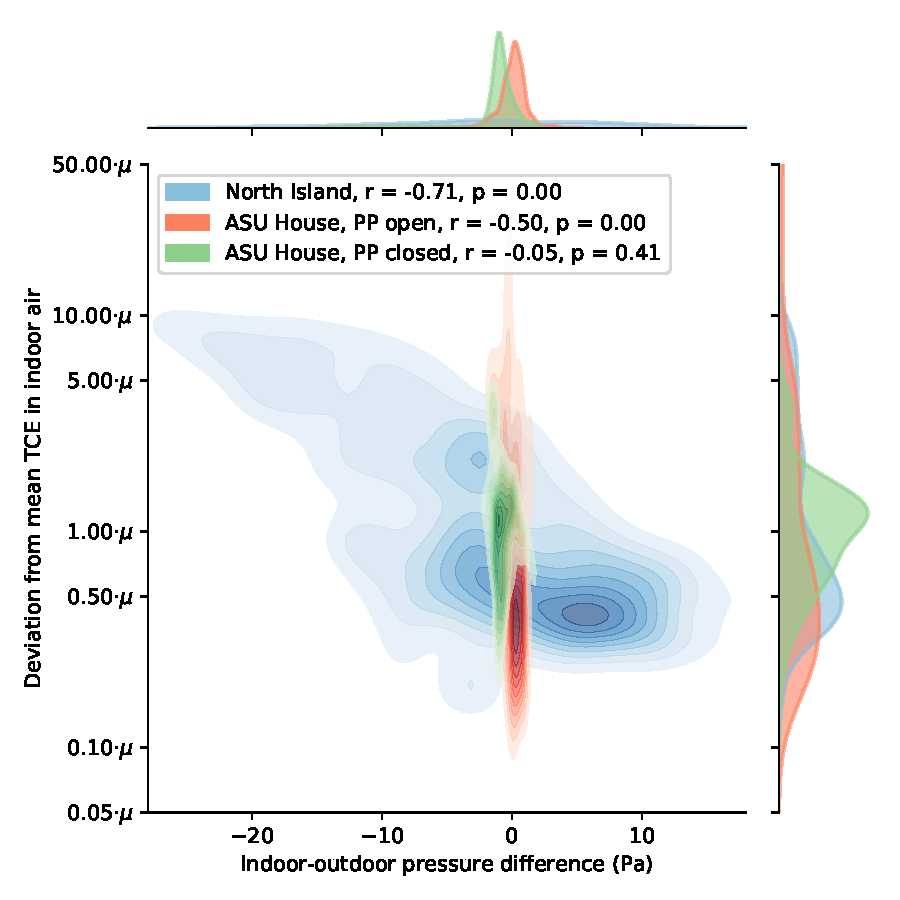
\includegraphics[width=\textwidth]{asu-nas.pdf}
\end{figure}

Figure \ref{fig:kde-asu-nas} show the result of the statistical analysis of the field data from the ASU and NAS North Island sites.  On the axes, the univariate KDE’s are shown.
The y-margin shows the distribution of the log-10 deviation from the mean TCE concentration in indoor air and the x-margin shows the distribution of indoor-outdoor pressure differences.
A negative pressure difference indicates that the structure is underpressurized, and thus air flows into the building, and a positive pressure difference indicates the opposite.
Thus the curves on the axis margins are the distribution functions of the respective measured variable values, considered independently.
They show the distributions of the results from the many different sampling events.
The distribution functions of pressure fluctuations are relatively simpler than those for the indoor air concentration measurements, and the pressure distribution functions for the pressure difference measurements at the ASU house are much simpler and narrower than that for comparable measurements at NAS North Island (see the distribution functions on the top margin of the figure).
Comparing the narrow red and green distribution functions for the ASU house results shows that whether the valve to the preferential pathway (PP) is open or not, roughly the same indoor-outdoor pressure differentials were seen.
This is not at all surprising, given that the existence of a preferential pathway buried beneath the foundation slab would not be expected to influence the indoor-outdoor pressure differential.
But when comparing the ASU house pressure differentials with those reported for the NAS North Island site (the blue distribution function), it is immediately apparent how much larger the pressure swings are at the latter site.
On this basis, if one associates contaminant entry rate with pressure differential alone, the NAS North Island site would be expected to show a much larger fluctuation in indoor air contaminant concentration than would the ASU house (but of course the preferential pathway changes the situation, as described below).

Turning to the univariate distributions for indoor air contaminant concentrations, the results show that even with the preferential pathway closed off, the results from the ASU house clearly show variations of an order of magnitude.
The construction of the KDE is naturally such that the overall distribution gives a mean of what is characterized as "$1.0 \mu$" in the figure, but around that mean the distribution of all measured concentrations falls within an order of magnitude of the mean.
The implication is that the most probable result from a single concentration sampling event will be a value around the mean, but the possibility that a single sampling event might give a result that is an order of magnitude higher or lower than a second independent sampling event cannot be ruled out, even under non-preferential pathway circumstances.
Thus, to the extent that the ASU house serves as a prototype for “normal” VI scenarios (when the preferential pathway was closed), it is only when any particular sampling event provides a result that is an order of magnitude below some action threshold that one can be highly confident that further sampling will not change this outcome.
The more sampling events that are involved, such that a population mean can confidently be estimated, the less likely that any future sampling event would give a value that is more than about a half an order of magnitude beyond that mean.
These are of course very rough rules of thumb, based upon this analysis of this data set.

When the preferential pathway beneath the ASU house is open, a very different picture emerges.
The calculated univariate distribution function takes on a much more complicated, somewhat bimodal character.
It should be recalled that the mean of all of the results remains, as before, at $"1.0 \mu"$.
The red distribution curve shows the origin of what has been reported as the “three orders of magnitude” variability in the indoor air contaminant concentrations.
On the one hand, there is a significant probability that any one measured concentration can be lower, up to even an order of magnitude below, the mean of the whole data set.
On the other hand, there is a spread to the upside of the mean by two orders of magnitude.
So in other words, the existence of an open preferential pathway in this case offers little guidance on what might be expected from any single sampling event.
This could easily have been inferred from the already raw published data from this site, but this analysis offers a statistical picture that suggests that there are distinctly different operational situations that give rise to different peaks in the observed distributions.
This, in turn, points to different operational parameters that have not yet been fully captured.

There is inherently greater spread in the ASU house data when the preferential pathway is open.
The variations in a direction greater than the mean show much greater spread, and arguably the choice of a Gaussian kernel is not necessarily the best.
The bivariate analysis below will shed more light on this point.

The univariate KDE distributions form the NAS North Island site show a distinctly bimodal distribution (the blue curve).
There is a population of sampling results above the mean and another below the mean.
Given that there was no influence of preferential pathways at this site, these results immediately flag the possibility that one is dealing with sample concentration populations that are strongly influenced by the other variable displayed on this plot - the indoor-outdoor pressure difference.
When the interior of the building is depressurized relative to ambient, there is a tendency towards indoor air contaminant concentrations higher than the mean, and when the building is pressurized, the values tend to fall below the mean.
This immediately suggests the examination of bivariate distributions, which are also shown on Figure \ref{fig:kde-asu-nas}, in the center of the plot.

The center of Figure \ref{fig:kde-asu-nas} shows the bivariate KDEs constructed based on the relationship between the two aforementioned variables.
The color-coding indicates the source of the dataset, with green again representing the ASU house dataset after the preferential pathway was closed, red is for before the pathway was closed, and blue the NAS North Island dataset.
The Pearson’s r-values and p-value for the relation between TCE in indoor air and indoor-outdoor pressure difference for each dataset are also shown.
The bivariate distributions in Figure \ref{fig:kde-asu-nas} show even more starkly the differences between the ASU house datasets and the NAS North Island dataset.
We believe that this is primarily due to the significant different indoor-outdoor pressure differences existing at these two sites.
Again, NAS North Island showed a much larger spread of indoor-outdoor pressure differential values, seen in the distributions on the top x-margin; the ASU house pressure difference distributions were quite Gaussian with a variation of just a few Pascals, whereas the NAS North Island distribution is rather more flat and includes a much larger span of values.

The bivariate distributions make clear one aspect of the ASU house results.
The “outlier” points at almost two orders of magnitude beyond the mean are associated with the existence of a preferential pathway and an unusually high indoor-outdoor pressure differential.
But for that particular combination of circumstances, the variability in indoor air contaminant concentrations, given existence of the preferential pathway, would have been “only” two orders of magnitude.
Comparing the green and red bivariate distributions, it is clear that the existence of the preferential pathway increases the potential spread of measured concentration values.
But beyond this, the correlation statistics show fairly convincingly that the pressure driving force is connected with the observed indoor air contaminant concentrations (even leaving out the few points at high depressurization), but that the correlation between indoor air contaminant concentration and pressure driving force is weak under “normal” VI conditions, where the preferential pathway was closed off.
This strongly suggests that under the latter conditions, advective entry was not a significant driver, and that ordinary diffusive processes were playing a role in bringing contaminant into the house from the area beneath the slab.
The above results reaffirm the problem that the potential existence of preferential pathways can cause for VI site investigations, i.e. they can greatly reduce the reliability of any single sampling event, requiring a larger number of samples to properly assess the site.
The existence of preferential pathways to the vicinity of a structure can enhance the effect of other variables, such as small pressure differences.
In this case, any single sampling event under “natural” conditions might give a value that is two orders of magnitude different from another sampling event.
Conservatism in that instance would suggest that any sampling results within two orders of magnitude of an action threshold would require re-sampling.
While the present results are taken from a single site, there is every reason to believe that this site can be representative of a large number of real sites.

Turning to the bivariate results for the NAS North Island site, the bivariate distributions leave little doubt that indoor-outdoor pressure differential is a key driver for measured indoor air contaminant concentrations.
The correlation statistics confirm the visual conclusion.
There is little surprise in the results, in that higher extents of depressurization lead to more contaminant entry.
Note that but for the portions of the blue contours at high and low pressure differences, the distribution of indoor air concentration values, relative to a mean, would be close to those from the ASU house.
In other words, at least some of the high temporal variability at NAS North Island comes from the rather extreme range of pressure differentials that exist there.
This supports a conclusion that under “normal” VI conditions, absent a preferential pathway, with the normally encountered pressure differentials of a few Pa, temporal variations in measured indoor air contaminant concentrations of an order of magnitude must be expected.
Clearly it would be useful to have a few more datasets from different sites to support such a general conclusion.

\begin{figure}[htb!]
  \caption{Probability density plots of the deviation from the mean Chloroform and Tetrachloroethene concentrations along with the indoor-outdoor pressure difference at the Indianapolis site}
  \label{fig:kde-indianapolis}
  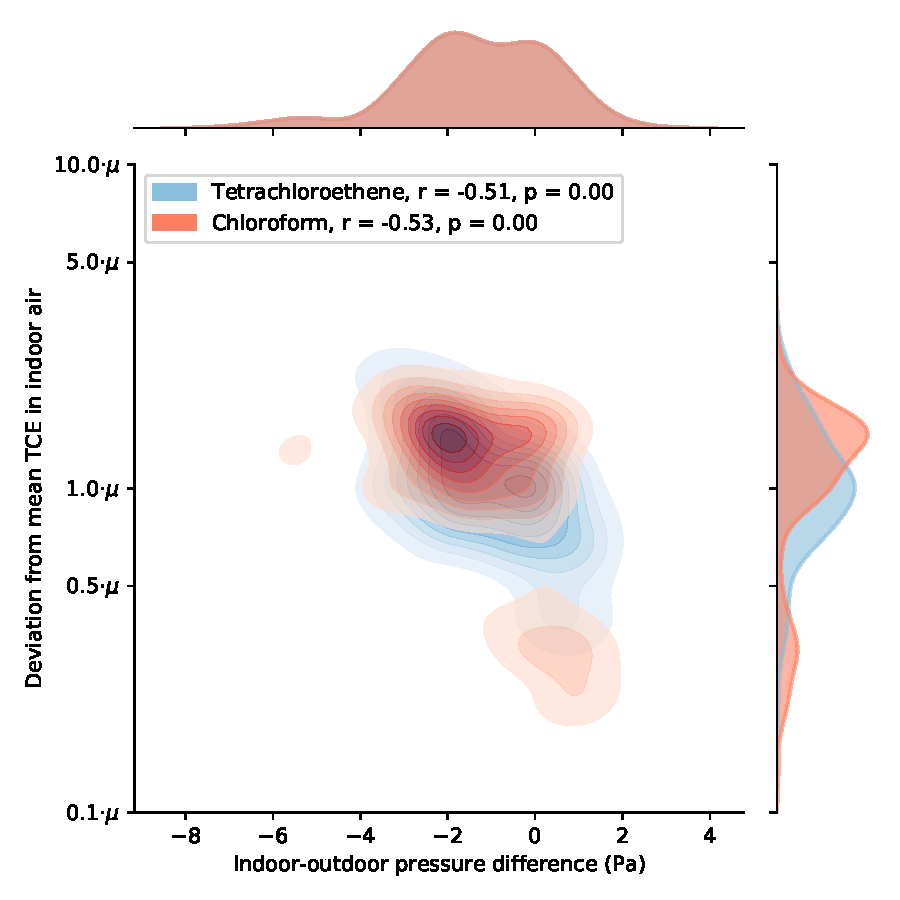
\includegraphics[width=\textwidth]{indianapolis-422.pdf}
\end{figure}

Figure \ref{fig:kde-indianapolis} shows the same as Figure \ref{fig:kde-asu-nas} but at the Indianapolis site, and the variations of Chloroform and PCE are considered instead of TCE.
The concentration of both Chloroform and PCE are still roughly equally log-normally distributed within half an order of magnitude above and below the mean, similar to the variation observed at the ASU house after the land drain was closed, as well as to the North Island site, if one would consider comparable indoor-outdoor pressure differences.
The distribution of pressure difference at the Indianapolis site is between that of ASU and North Island, with the structure there typically being more depressurized than ASU but less than North Island.
The relationship between pressure difference and IACC is much stronger at the Indianapolis site than it was at the ASU house, but less so than at North Island.
Given what is known about the soil around Indianapolis site, this is somewhat surprising, as it is not significantly different from the ASU site (which North Island is).
This may be evidence of the interaction with the PP that exists at the site, although the extreme variations in IACC cannot be observed here.
\end{comment}

\subsubsection{The Role Of Air Exchange Rate}
% Air exchange rate plots
\begin{figure}[htb!]
  \caption{Comparison between the recorded  and the calculated TCE in indoor air at the ASU house, assuming constant air exchange rate. \ref{fig:asu-iacc-ae-overview} shows the TCE in indoor air across time as well as the exchange rate. \ref{fig:violin-iacc-aet} shows the distribution of these values for three periods.}
  \label{fig:ae-analysis}
  % "Overview" plot
  \begin{subfigure}{\textwidth}
    \caption{ }
    \label{fig:asu-iacc-ae-overview}
    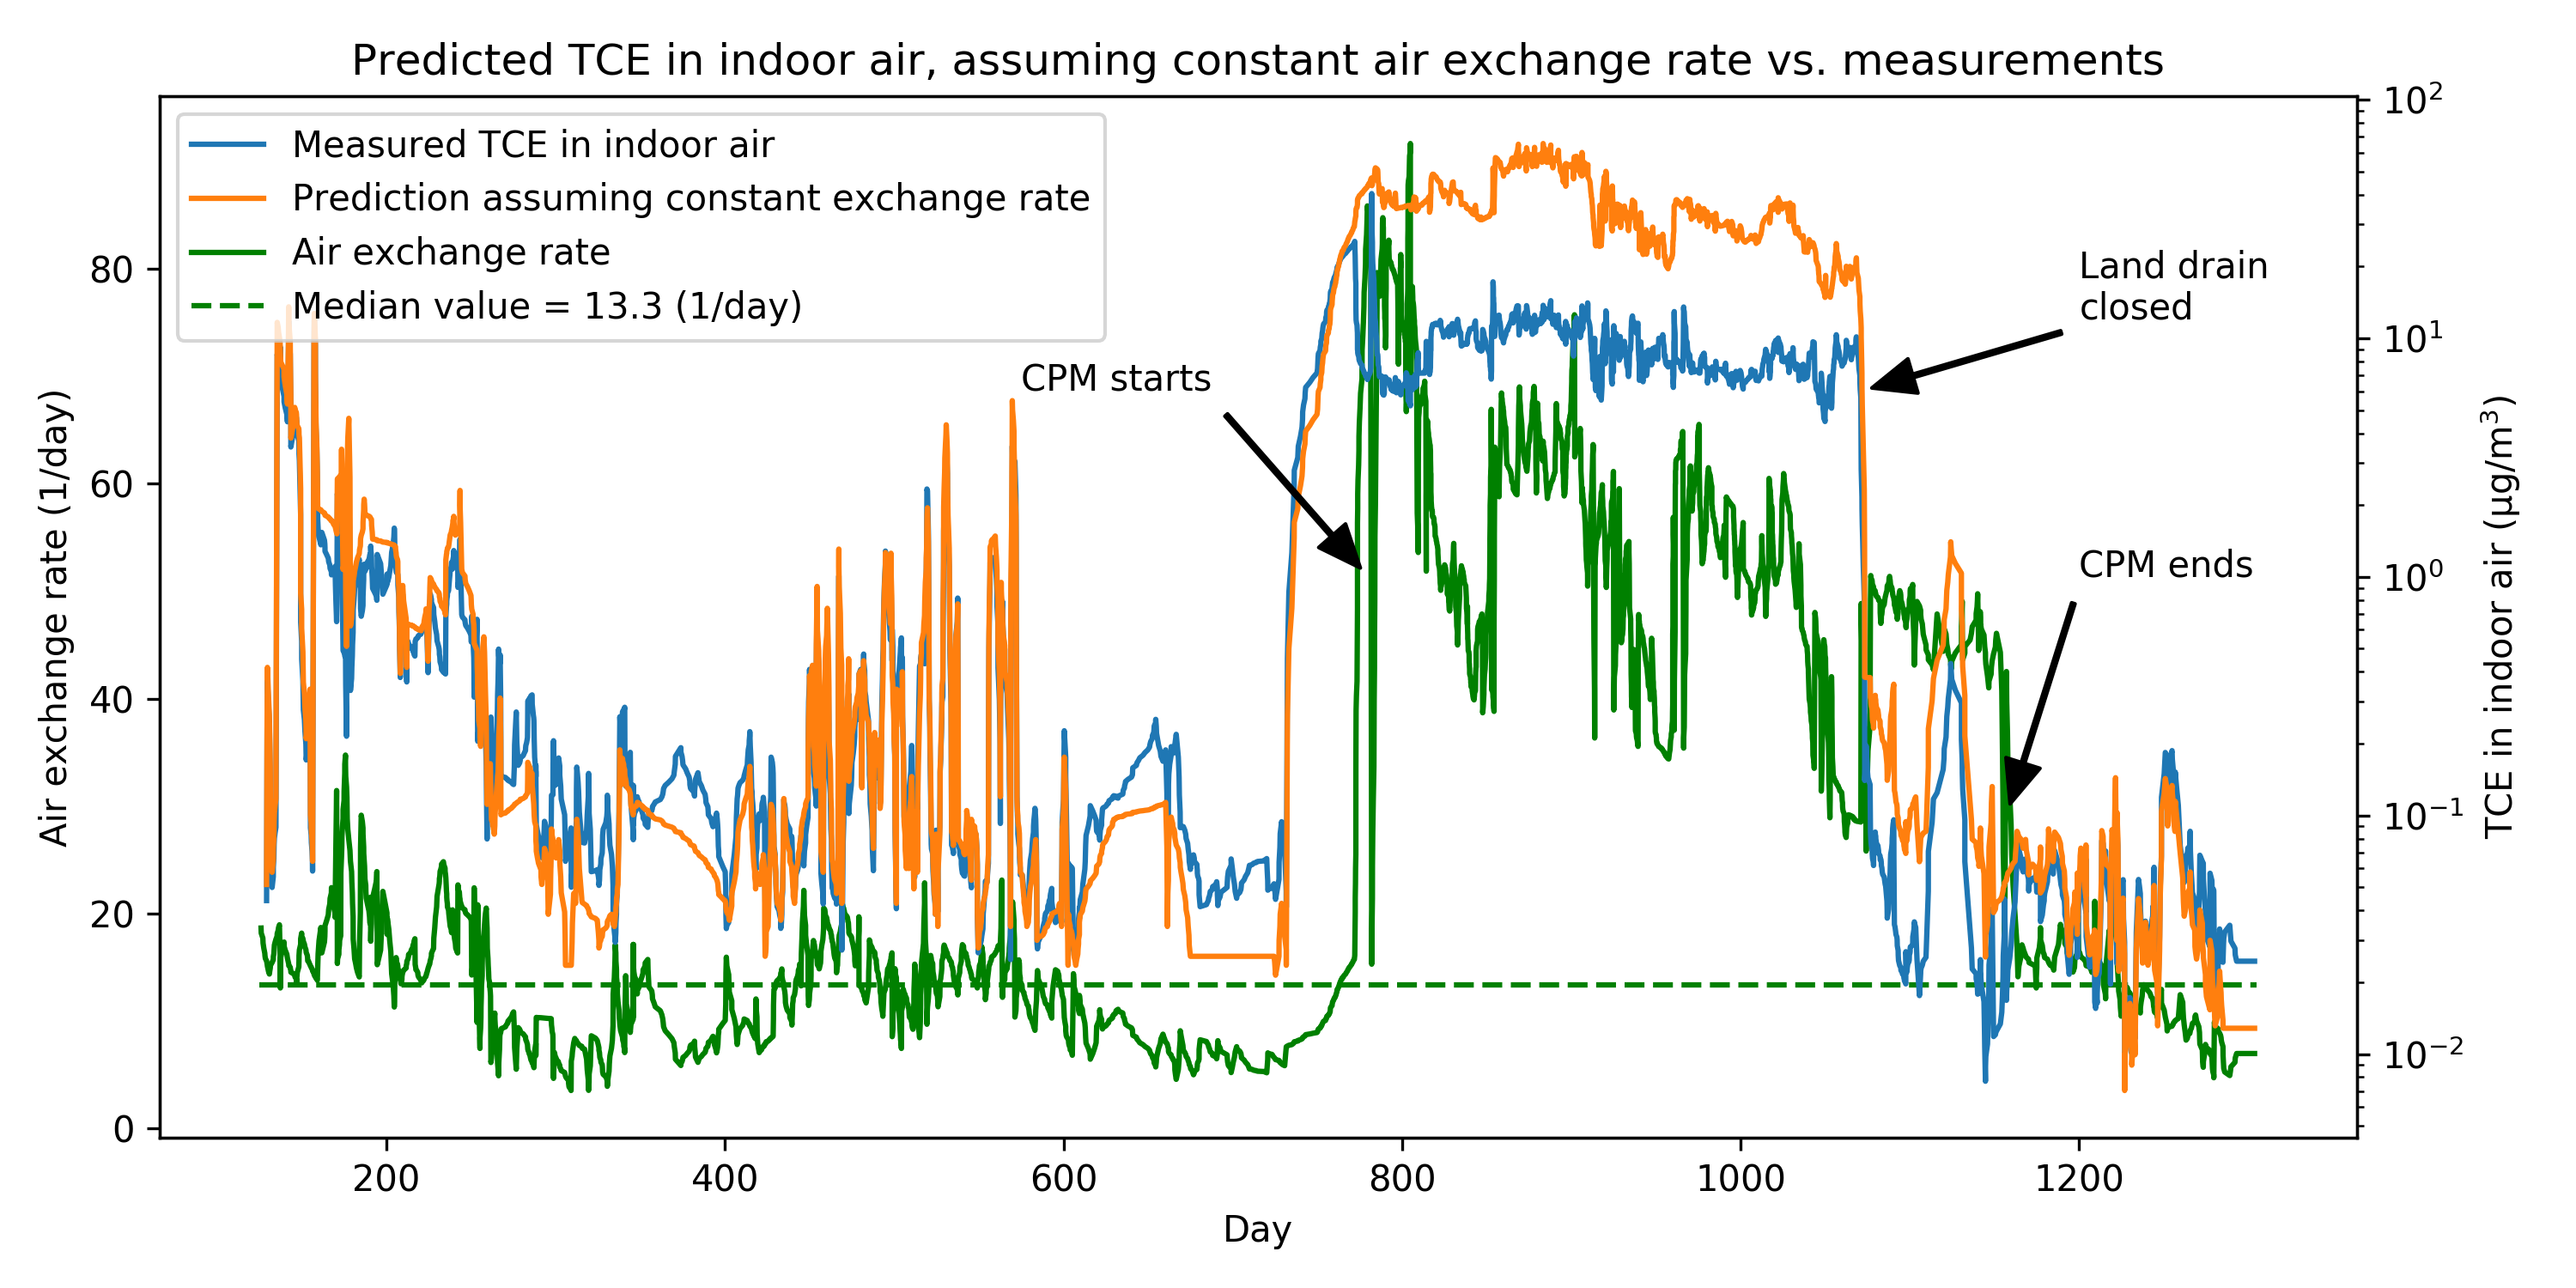
\includegraphics[width=\textwidth]{asu-iacc-ae-overview.png}
  \end{subfigure}
  % Violinplot figure
  \begin{subfigure}{0.75\textwidth}
    \caption{ }
    \label{fig:violin-iacc-aet}
    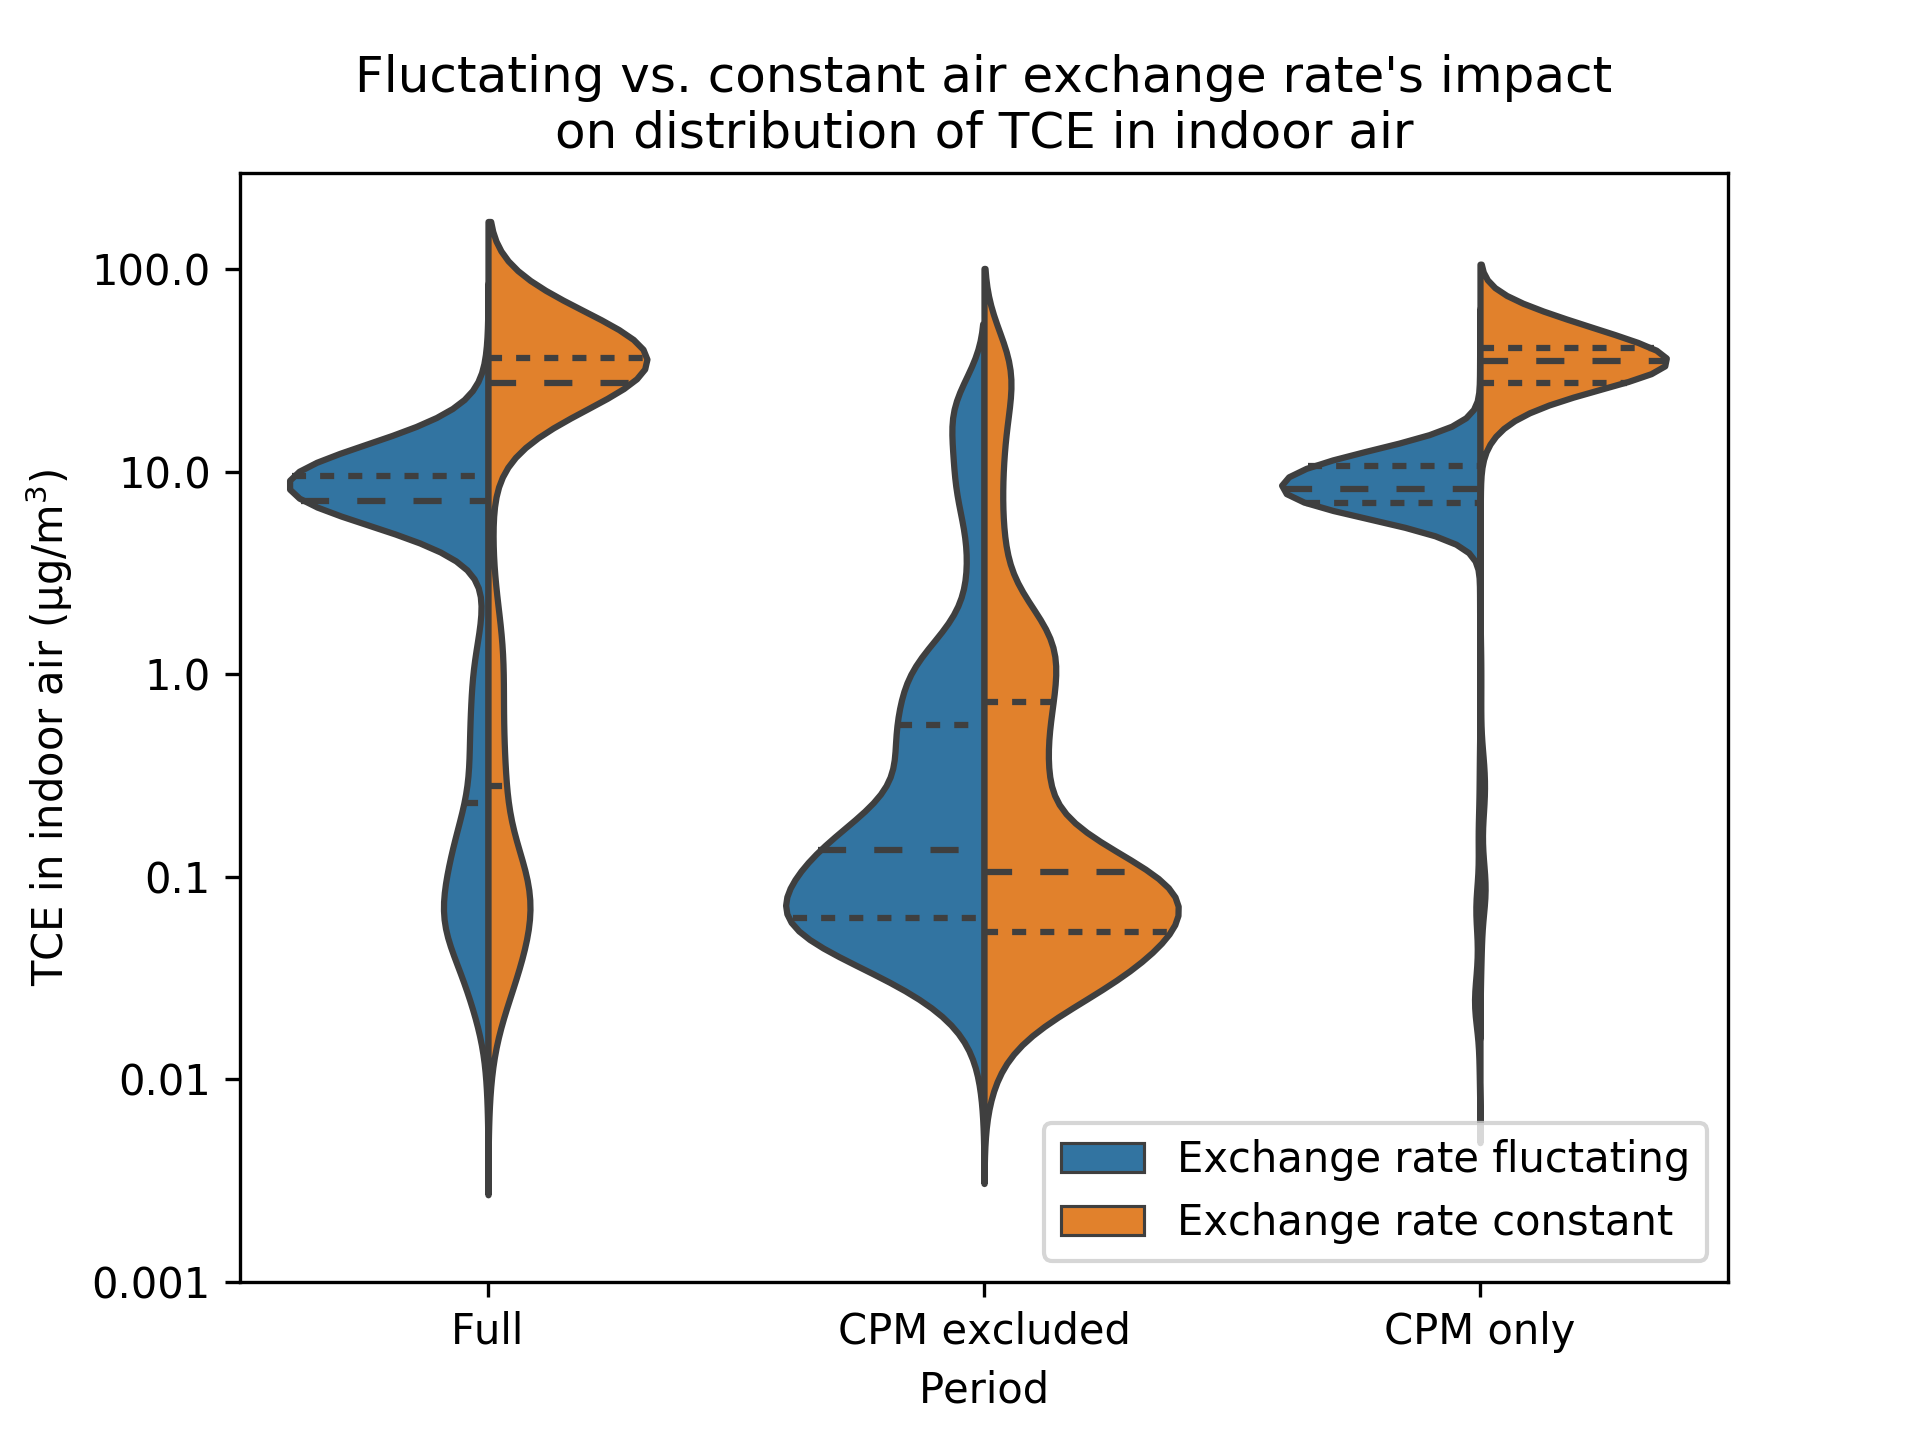
\includegraphics[width=\textwidth]{violin-asu-iacc.png}
  \end{subfigure}
\end{figure}
Air exchange rate, which measures how often the interior air in a given building is exchanged with exterior air, is the main parameter characterizing contaminant expulsion, and another highly dynamic process.
Exploring the impact of fluctuations in air exchange rate is thus also important for the development of sampling strategies.
At the ASU house, the contaminant entry rate into the structure (called emission rate in that study) as well as the building air exchange rate were recorded across time.
This allows for exploration of the impact that fluctuating air exchange rate has on the final IACC by solving the CST equation, using the recorded contaminant entry rate as one input, and assuming a constant air exchange rate.
The rationale is to show the extent of variability in IACC due to factors other than fluctuations in air exchange rates.
We have taken this factor out of consideration by assuming a single constant exchange rate, characteristic of the whole period.

In Figure \ref{fig:asu-iacc-ae-overview}, the measured IACC and air exchange rate across time are shown, with the predicted IACC assuming a constant air exchange rate.
The median air exchange rate value for the pre-CPM period was chosen as this seemed to be the most representative value for this time period.
From Figure \ref{fig:asu-iacc-ae-overview} it may be seen quite clearly that for the non-CPM periods, the calculated IACC assuming constant and actual fluctuating exchange rates are quite similar.
In other words, in this instance it is unlikely that the variations in IACC were driven by fluctuations in air exchange rate.

This is more clearly shown in Figure \ref{fig:violin-iacc-aet}, where KDEs of the IACC are constructed assuming the constant and fluctuating air exchange rate cases.
This figure shows the relative probability of being at a particular TCE in indoor air concentration at the ASU house.
These are compared to each other for 1. the full measurement period, 2. the non-CPM periods and 3. the CPM period.
Looking at the full period, it does not appear as though the two cases of steady and fluctuating air exchange rate are comparable, the distribution functions for IACC are different and offset.
The curves to the different sides of the vertical line for the "full" measurement period represent the probability distributions for the indicated values of IACC.
It appears as though assuming a constant air exchange rate shifts the IACC probability distribution to higher values.
The reason for this are more apparent when considering the CPM and non-CPM periods separately.

Considering only the CPM period, assuming a constant air exchange rate does not influence the shape of the IACC distribution, but assuming constant exchange rate shifts the IACC to a higher values.
This is because the actual air exchange rate for this CPM period is significantly higher than the assumed median value, and much more contaminant is actually exchanged with the exterior.
The shape of the IACC distribution is not very different from that which takes the air exchange fluctuations into account however, indicating that fluctuating exchange rate is not a major contributor to observed IACC variation for this period (the distinction being drawn between variation and absolute levels of IACC).

The non-CPM period is the condition under which field practitioners would normally collect samples at a VI site.
It is clear here that there is only a very minor difference made in assuming a constant vs. real fluctating air exchange rate, again indicating that account for the minor fluctuations of air exchange rate's impact on variations in IACC is not important.
\citeauthor{rackes_time-averaged_2016}\cite{rackes_time-averaged_2016} drew similar conclusions regarding the relationship between IACC and air exchange rate.

\subsection{The Influence of Preferential Pathways}

% Point is:
% If preferential pathways exist, then roughly 1-3 orders of magnitude variability are possible.

% Definition: A preferential pathway is a pathway that allows for contaminant vapor to enter a structure directly or close to the building - circumventing much of the resistance to transport in the soil.

% How do I deal with this? How do I know if preferential pathways may be an issue?

% Scenario: Preferential pathway directly connected to the building.
% - Identify sewer & plumbing fixtures.
% - Drains and sumps may be sources.

% Scenario: Preferential pathway in the near slab area.
% - Permeable sub-base necessary.
% - May have a limited “sphere of influence”.
% -- Limit likely not reached for a normal house.
% -- Limit more likely to be reached for larger structures.

% Relevant for both: Check local manhole/sewer for presence of contaminant - likely source for the preferential pathway.

\subsubsection{Conclusions From Steady-State Modeling}

\begin{figure}[htb!]
  \caption{Sensitivity analysis of IACC dependence on indoor/outdoor pressure difference for a model featuring a PP (\ref{fig:ss-sensitivity-analysis-pp}) and without a PP (\ref{fig:ss-sensitivity-analysis-no-pp}). Results compared with field data from ASU house.}
  \label{fig:ss-sensitivity-analysis}
  % "Overview" plot
  \begin{subfigure}{0.55\textwidth}
    \caption{PP present. Sensitivity to the presence of a gravel sub-base and contamination in the PP considered.}
    \label{fig:ss-sensitivity-analysis-pp}
    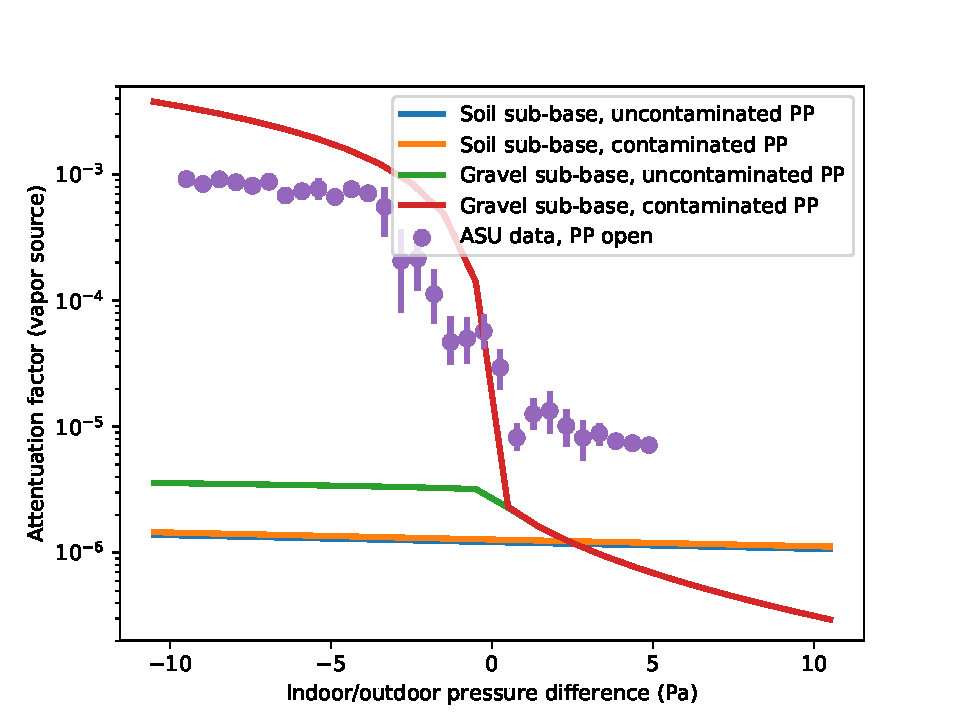
\includegraphics[width=\textwidth]{yes-pp.pdf}
  \end{subfigure}
  % Violinplot figure
  \begin{subfigure}{0.55\textwidth}
    \caption{No PP preseent. Sensitivitiy to the presence of a gravel sub-base considered.}
    \label{fig:ss-sensitivity-analysis-no-pp}
    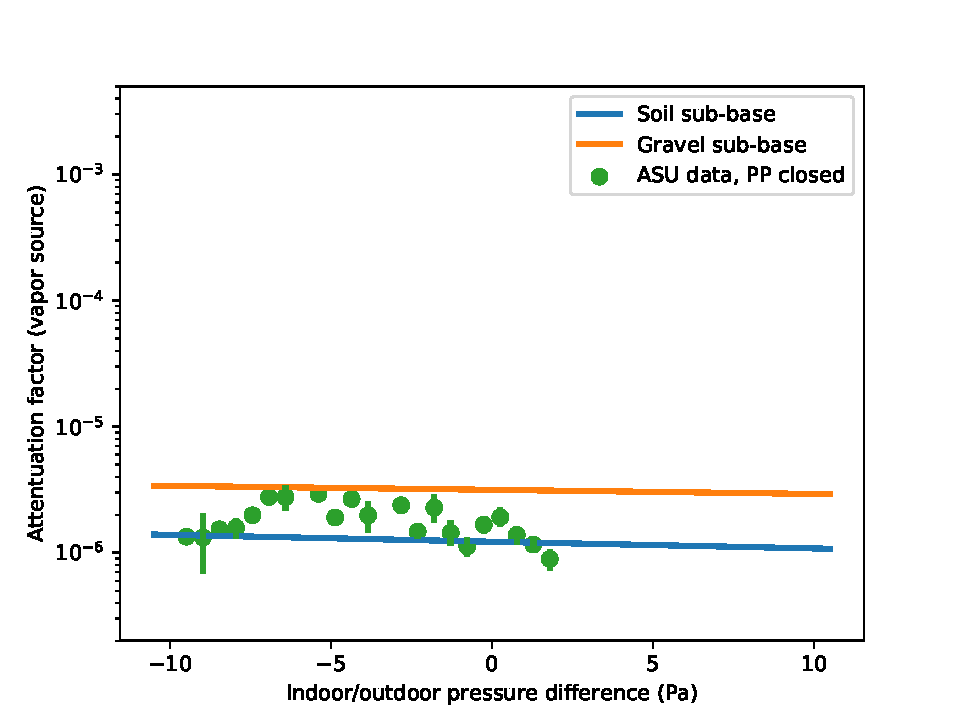
\includegraphics[width=\textwidth]{no-pp.pdf}
  \end{subfigure}
\end{figure}

\begin{comment}

Clearly, PPs pose a major problem for site investigations, in particular because they may be difficult or even impossible to anticipate or uncover; even at a well studied site like the ASU house it took years to discover the PP.
Therefore, there is a need to consider other indications that a PP is present.

% Sensitivity analysis plot showing when a PP is relevant
\begin{figure}[htb!]
  \caption{Attenuation factor relative to contaminant vapor in equilibrium with groundwater as a function of indoor-outdoor pressure difference. The effects of a preferential pathway, that is either contaminated or uncontaminated as well as that of having a gravel sub-base vs. uniform sandy clay soil are considered.}
  \label{fig:model_results_sensitivity_analysis}
  % Upper left
  \begin{subfigure}[t]{0.45\textwidth}
    \caption{ }
    \label{fig:model_results_sensitivity_analysis_0}
    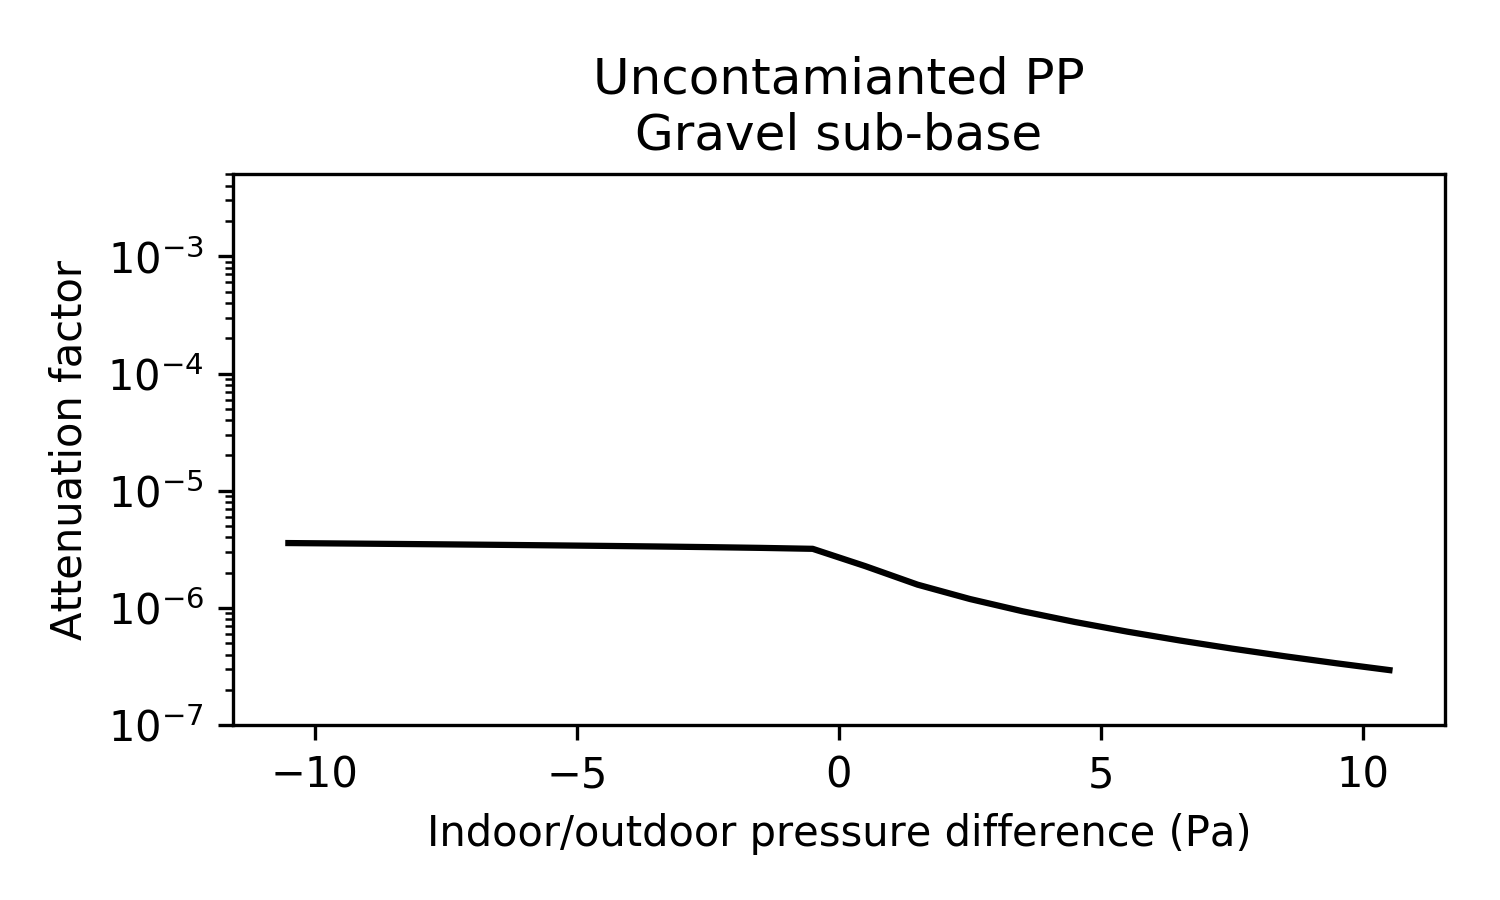
\includegraphics[width=\textwidth]{ss_pp_sensitivity_analysis_0.png}
  \end{subfigure}
  % Upper right
  \begin{subfigure}[t]{0.45\textwidth}
    \caption{ }
    \label{fig:model_results_sensitivity_analysis_1}
    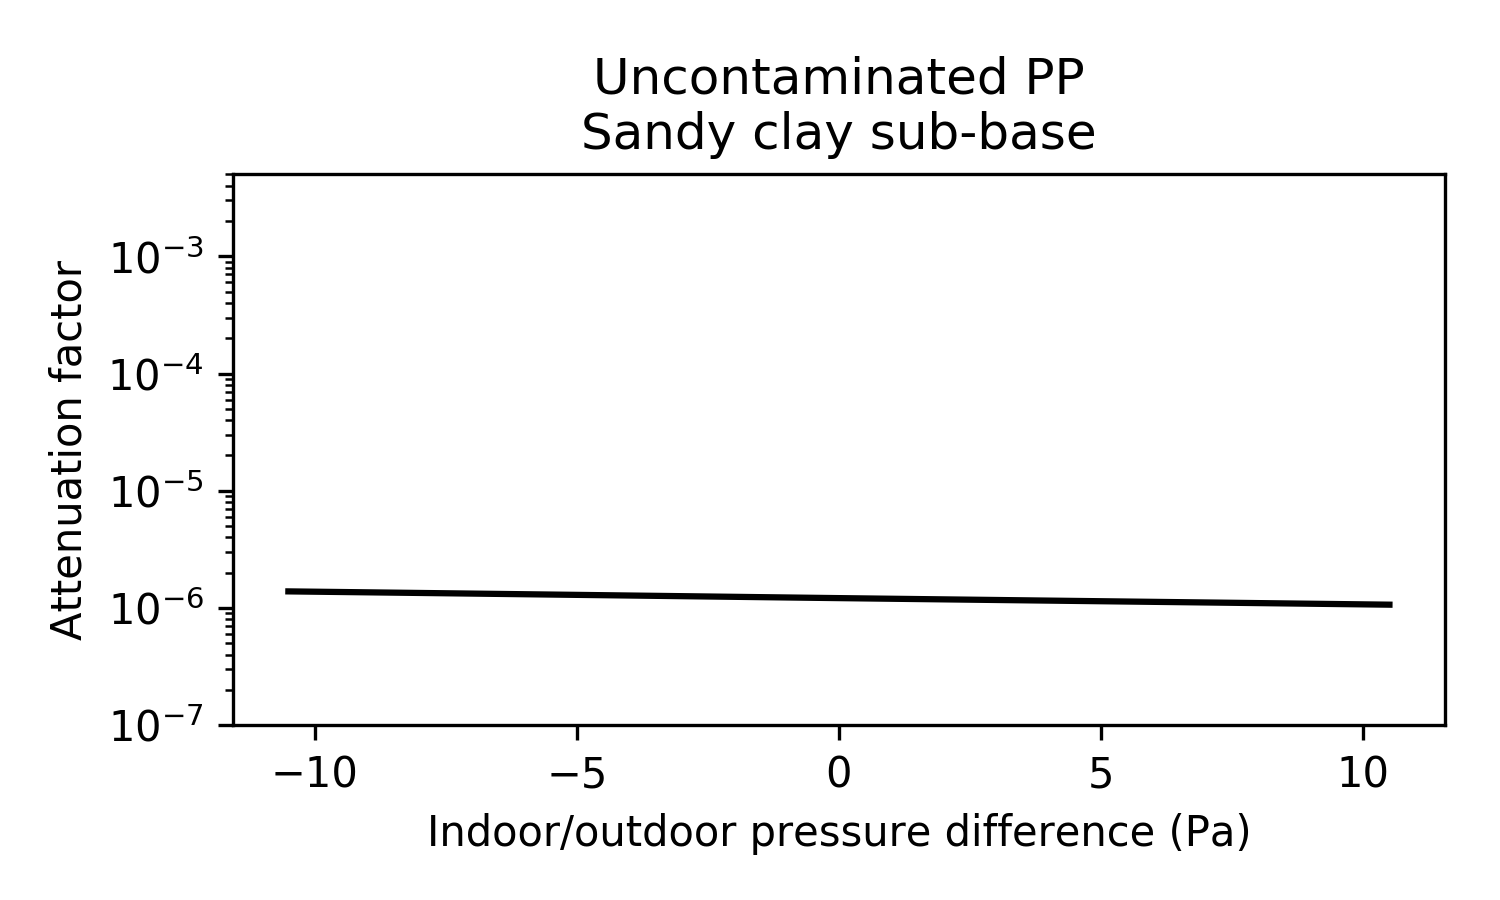
\includegraphics[width=\textwidth]{ss_pp_sensitivity_analysis_1.png}
  \end{subfigure}
  % Middle left
  \begin{subfigure}[t]{0.45\textwidth}
    \caption{ }
    \label{fig:model_results_sensitivity_analysis_2}
    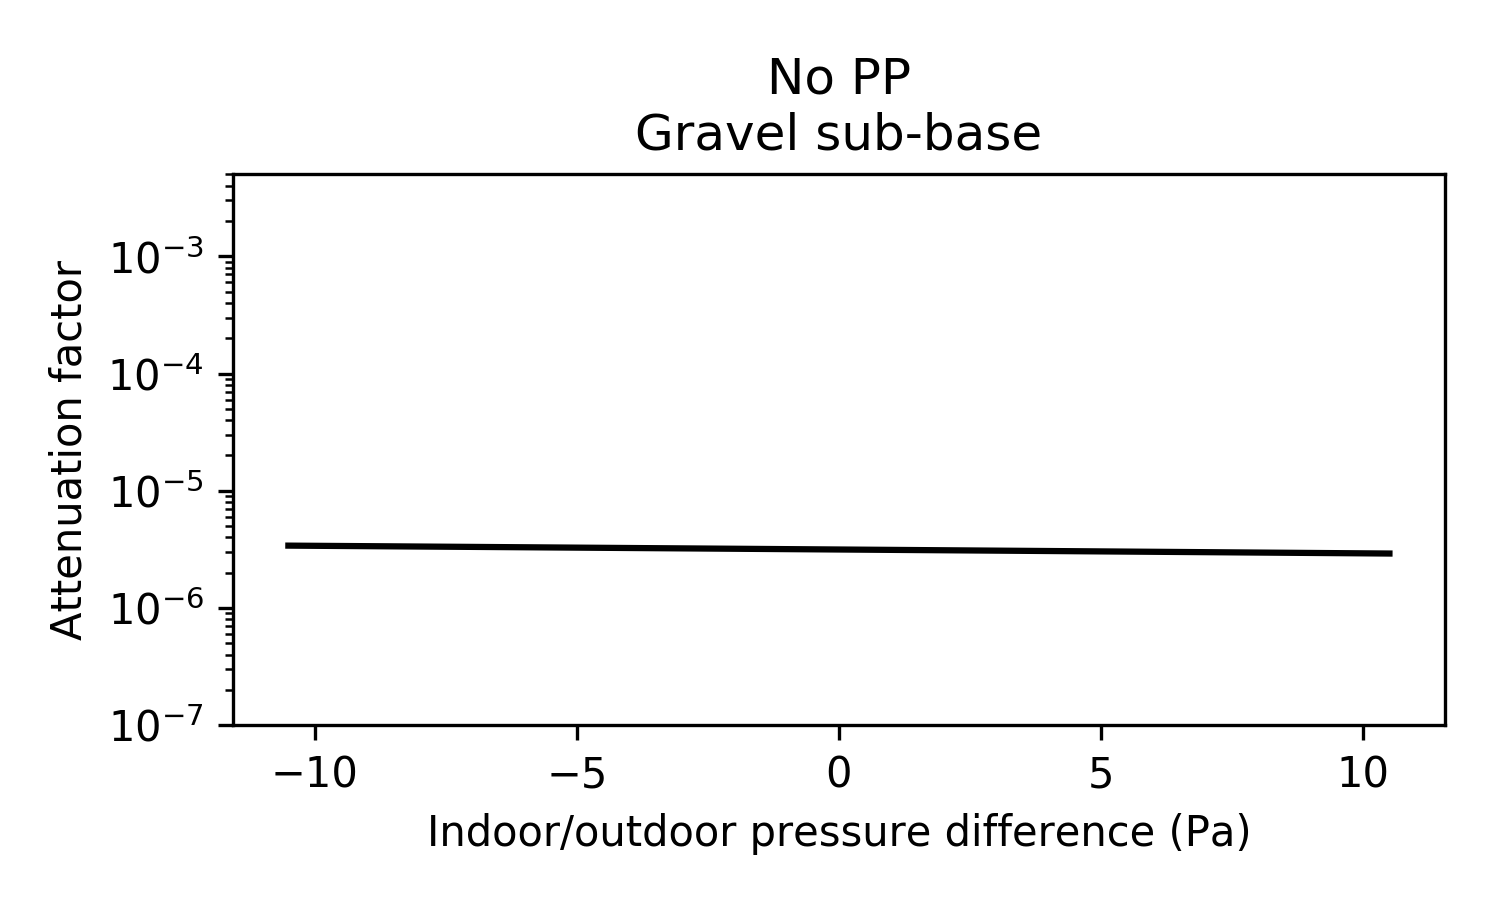
\includegraphics[width=\textwidth]{ss_pp_sensitivity_analysis_2.png}
  \end{subfigure}
  % Middle right
  \begin{subfigure}[t]{0.45\textwidth}
    \caption{ }
    \label{fig:model_results_sensitivity_analysis_3}
    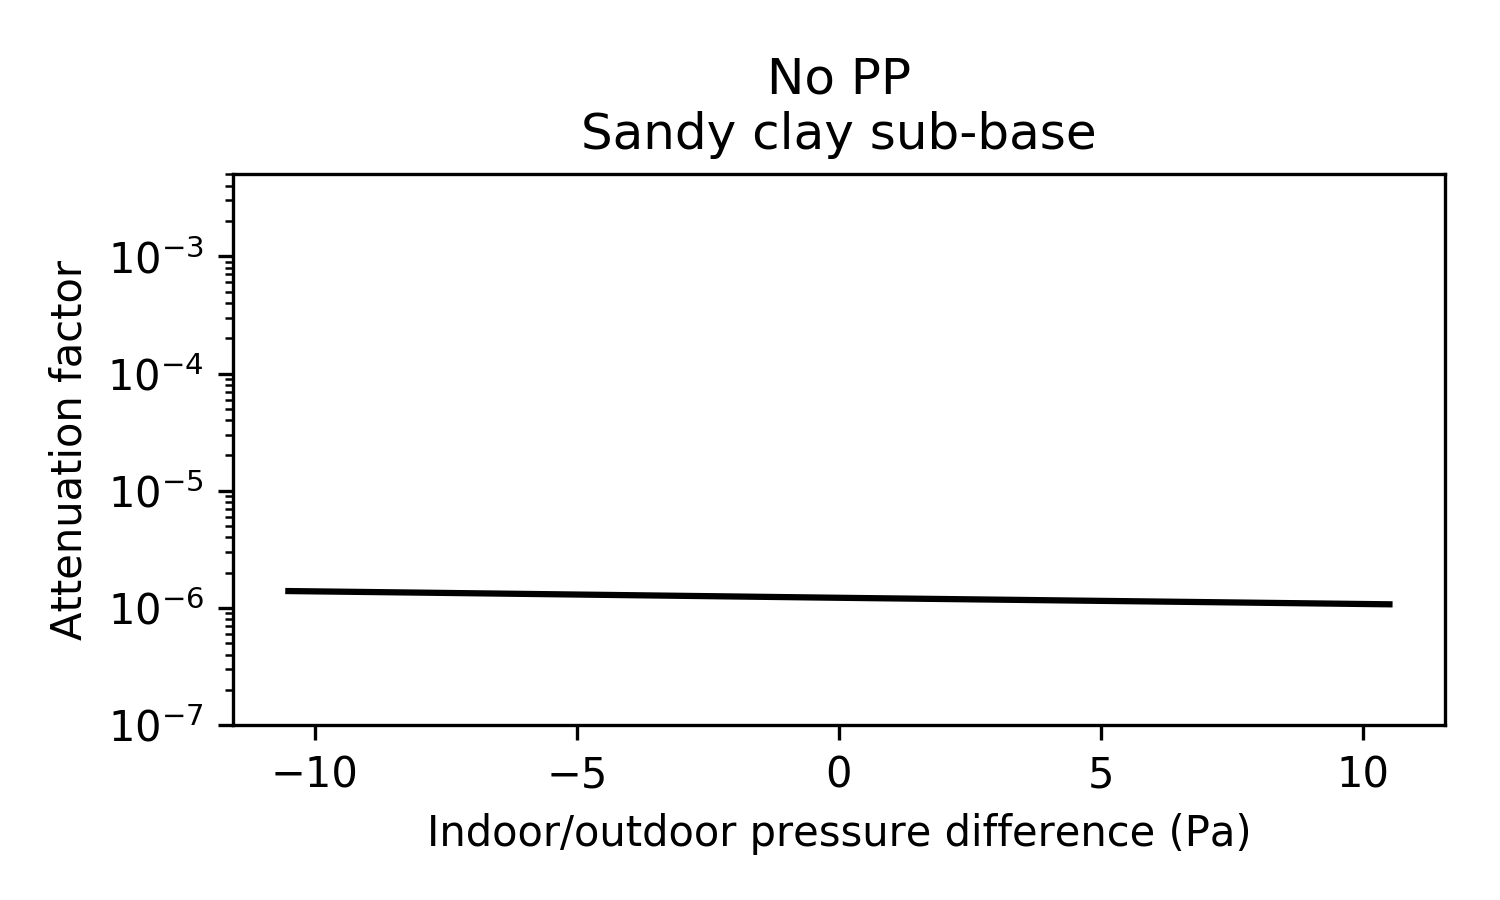
\includegraphics[width=\textwidth]{ss_pp_sensitivity_analysis_3.png}
  \end{subfigure}
  % Lower left
  \begin{subfigure}[t]{0.45\textwidth}
    \caption{ }
    \label{fig:model_results_sensitivity_analysis_4}
    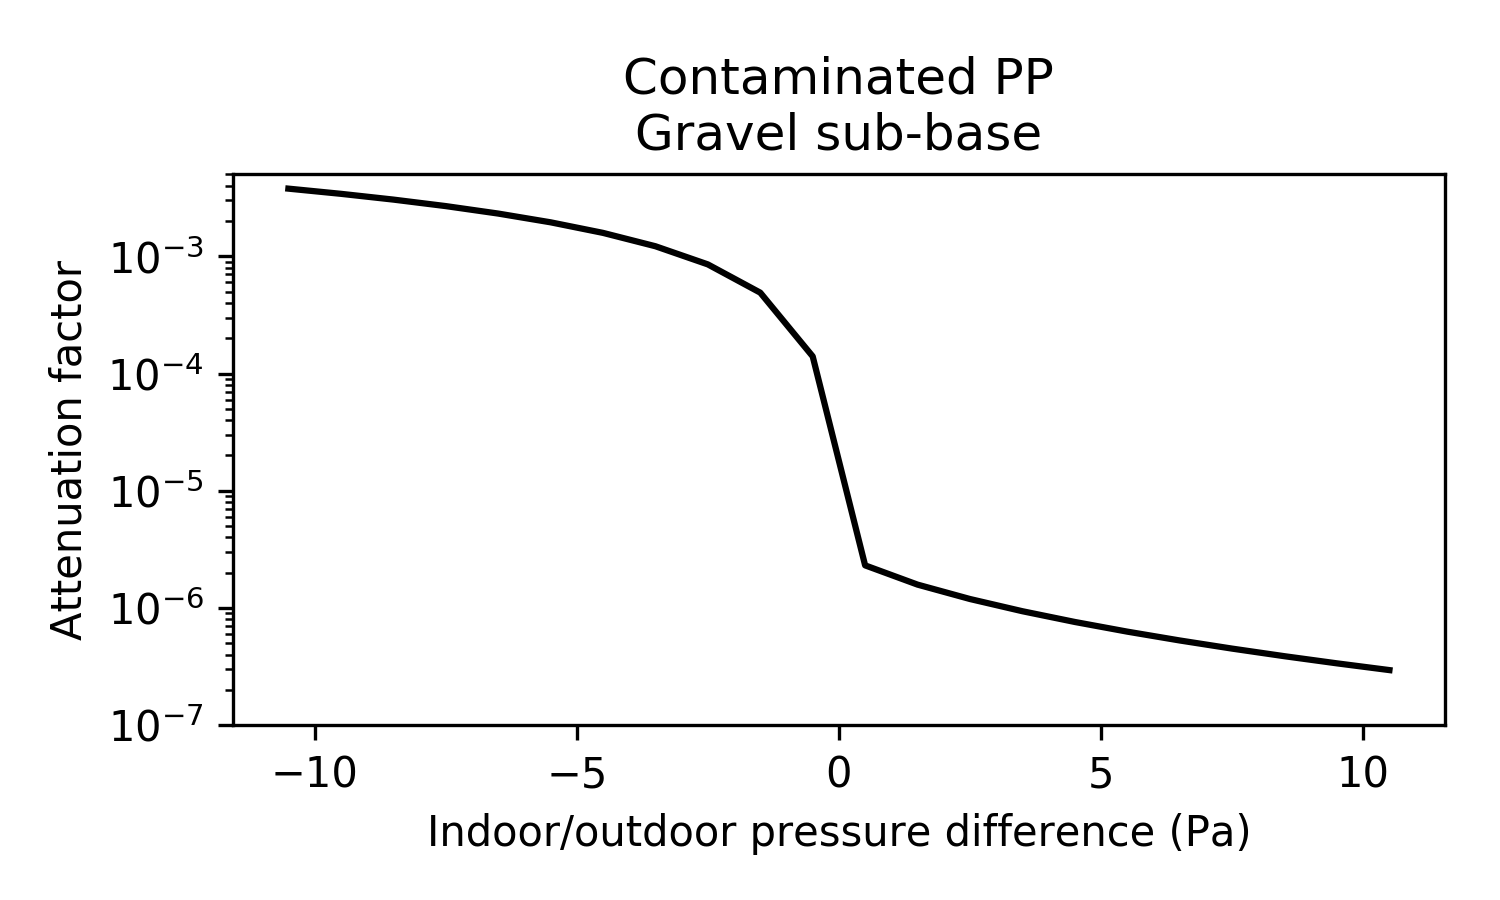
\includegraphics[width=\textwidth]{ss_pp_sensitivity_analysis_4.png}
  \end{subfigure}
  % Lower right
  \begin{subfigure}[t]{0.45\textwidth}
    \caption{ }
    \label{fig:model_results_sensitivity_analysis_5}
    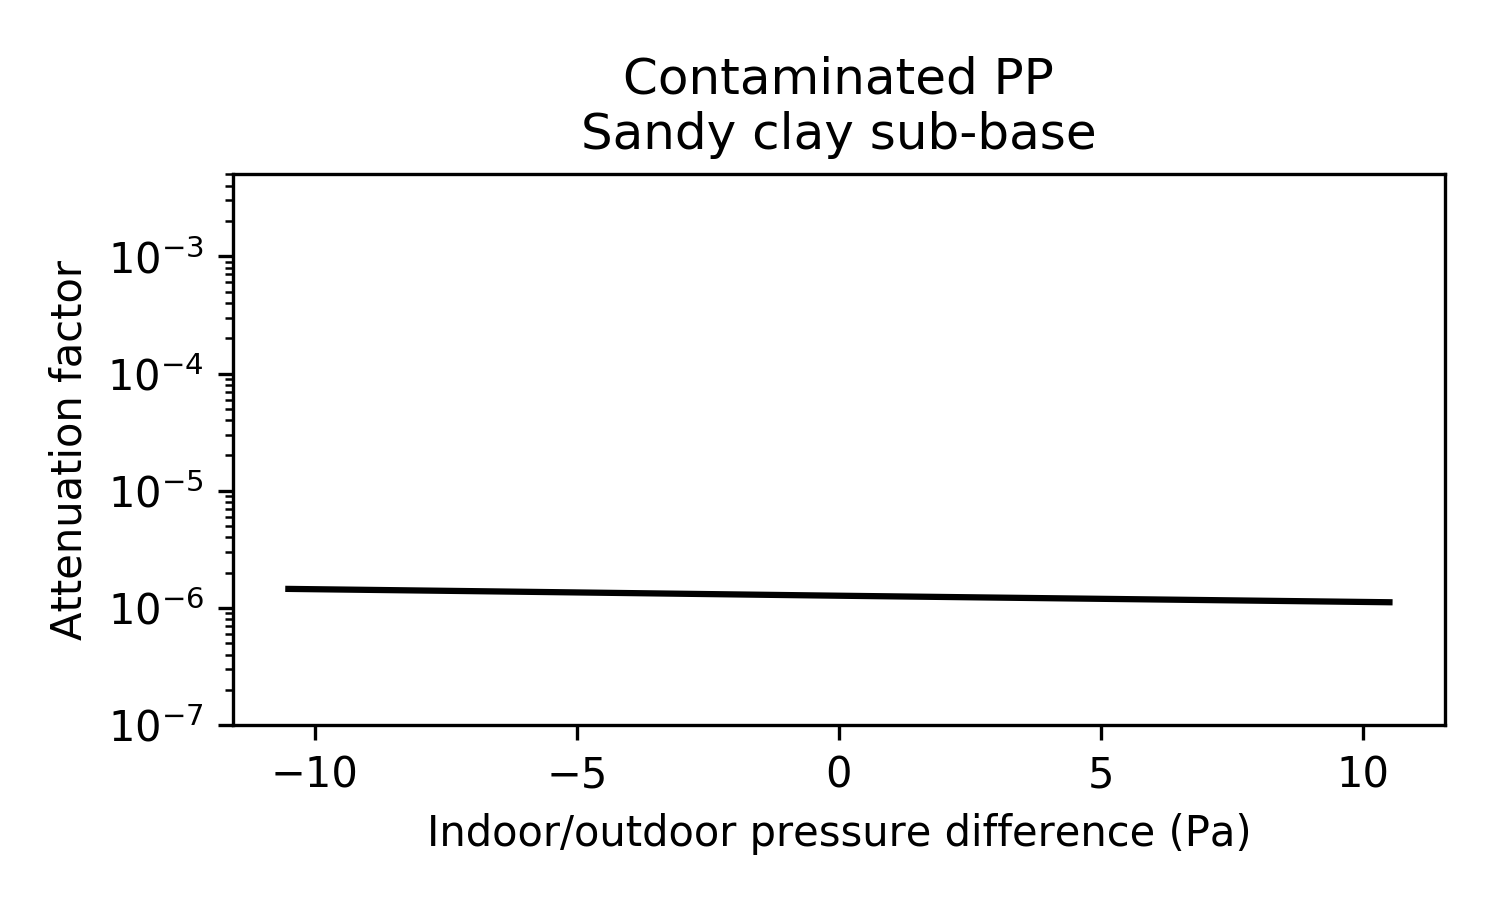
\includegraphics[width=\textwidth]{ss_pp_sensitivity_analysis_5.png}
  \end{subfigure}
\end{figure}

One way has been suggested by the situation at the ASU house, where there clearly was a PP containing contaminant vapor, and the PP exited into a gravel (permeable) sub-base.
This situation can be examined using the VI model introduced earlier by examining how IACC is impacted by various factors over a range of indoor-outdoor pressure difference values.
Instead of representing IACC as absolute concentration, we now non-dimensionalize with respect to the vapor in equilibrium with the groundwater contaminant concentration.
This non-dimensionalized property is commonly called the attenuation factor and is denoted by $\alpha_\mathrm{gw}$.
The result of a sensitivity analysis relative to several factors is seen in Figure \ref{fig:model_results_sensitivity_analysis}.
These examine scenarios in which the indoor-outdoor pressure difference is a driver for VI.

In this figure, all the graphs in the left column show results for a scenario, in which the house has a gravel sub-base, with the remaining surrounding soil assumed to be sandy clay.
All the right column graphs features only sandy clay soil, directly in contact with the slab.
Figure \ref{fig:model_results_sensitivity_analysis_0} considers an uncontaminated PP ($\chi = 0$), i.e. the PP delivers clean air to beneath the slab.
In \ref{fig:model_results_sensitivity_analysis_1} there is no PP present at all, giving a reference state for a "normal" VI scenario.
\ref{fig:model_results_sensitivity_analysis_2} features a contaminated PP ($\chi = 1$), i.e. the PP delivers contaminant vapor at a concentration characteristic of underlying groundwater.

In terms of conditions that may lead to significant temporal transients in $\alpha_\mathrm{gw}$, driven by indoor-outdoor pressure difference, most of the cases in this analysis show negative results.
There are only two combinations of factors where significant changes in $\alpha_\mathrm{gw}$ accompany the changes in indoor-outdoor pressure difference, both involving the permeable (gravel) sub-base into which a PP enters.
In \ref{fig:model_results_sensitivity_analysis_2}, the PP is filled with contaminant vapor whereas figure \ref{fig:model_results_sensitivity_analysis} involves the PP only delivering "clean" air to the gravel sub-base.
When the building is overpressurized (positive indoor-outdoor pressure difference), the two cases exhibit similar behavior, i.e. $\alpha_\mathrm{gw}$ is low as expected.

When the building is underpressurized, the uncontaminated PP case involves barely any increase in $\alpha_\mathrm{gw}$ while there is a very significant increase in $\alpha_\mathrm{gw}$ in the contaminated PP case.
For the contaminated PP scenario, this is quite easy to understand, as the extra air flow provided by the PP into the gravel sub-base very effectively disperses contaminant vapor across the sub-base and the contaminant entry rate is increased.

When the PP is provides clean air, the increase in air flow into the sub-base with depressurization is the same.
However, the resulting increase in air entry rate does not bring in more contaminant as clean air is being drawn in.
This means that most of the contaminant entry rate is still only controlled by the usual process of diffusion through the soil, giving a result that is actually similar to that for the "no PP and with gravel sub-base" scenario.
Thus, for a PP to be a significant contributor to contaminant entry at a VI site the conditions such as featured in the bottom left case are required, i.e. a permeable sub-base and the PP must be a source of contaminant.

Various techniques for determining the potential for sewer gas entry into a house are described by \citeauthor{nielsen_remediation_2017-1}\cite{nielsen_remediation_2017-1}.
Collecting contaminant vapor samples from nearby manholes is also recommended, however one should be aware that contaminant vapors can potentially travel very long distances in a sewer system\cite{mchugh_evidence_2017,roghani_occurrence_2018,riis_vapor_2010}.

% Models specific to ASU & North Island
\begin{figure}[htb!]
  \caption{Attenuation factor vs. indoor-outdoor pressure difference when considering VI scenarios similar to the ASU house and the North Island NAS site (\ref{fig:ss_asu} and \ref{fig:ss_north_island} respectively).}
  \label{fig:model_results_asu_north_island}
  % ASU
  \begin{subfigure}[t]{0.45\textwidth}
    \caption{ }
    \label{fig:ss_asu}
    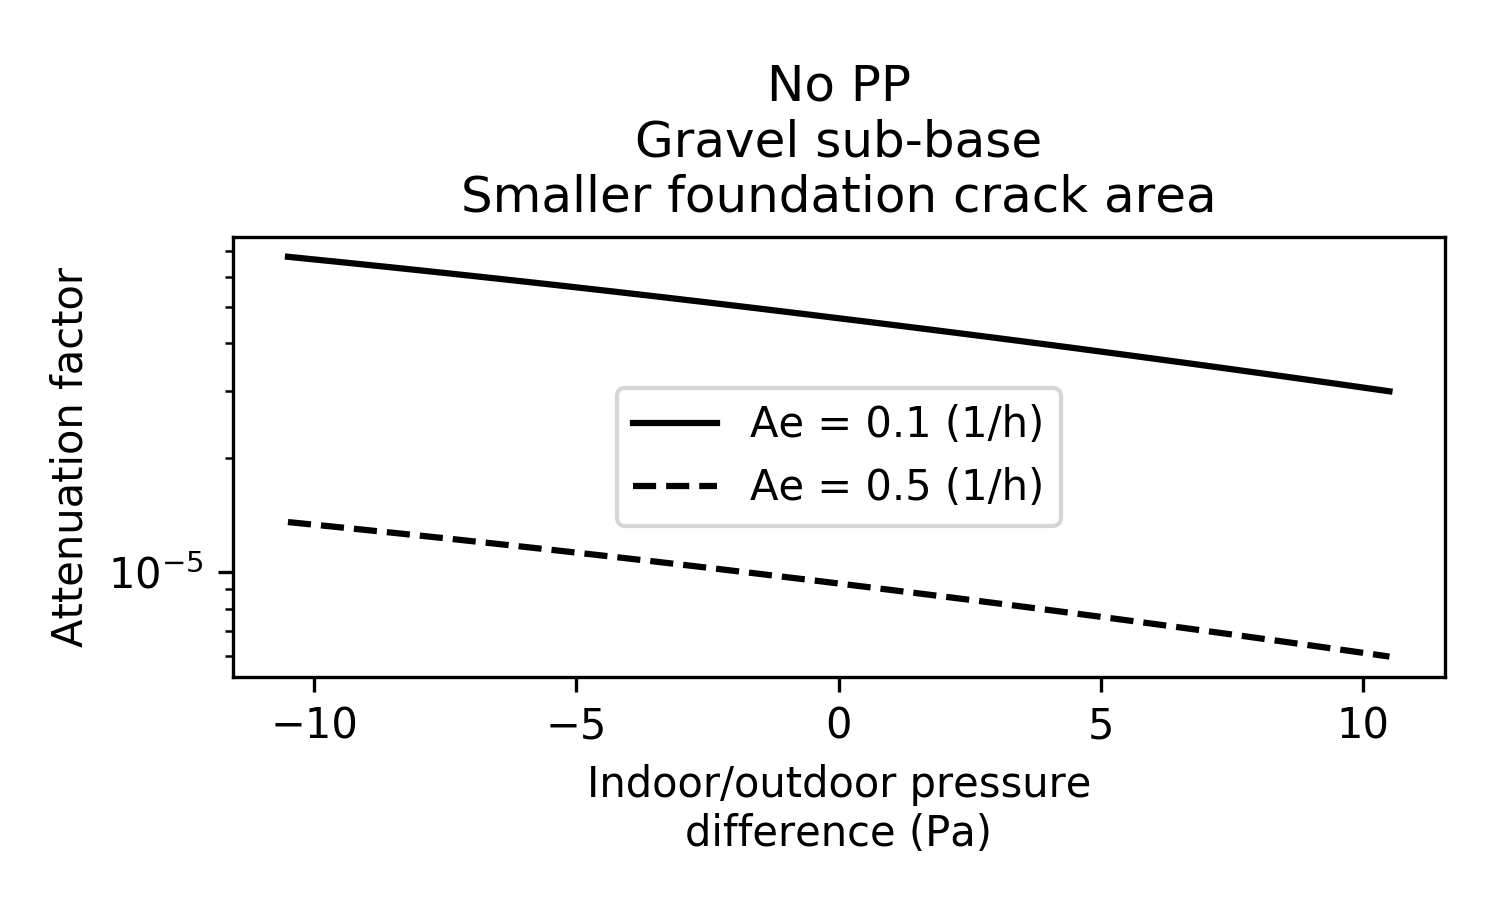
\includegraphics[width=\textwidth]{ss_asu.png}
  \end{subfigure}
  % North Island
  \begin{subfigure}[t]{0.45\textwidth}
    \caption{ }
    \label{fig:ss_north_island}
    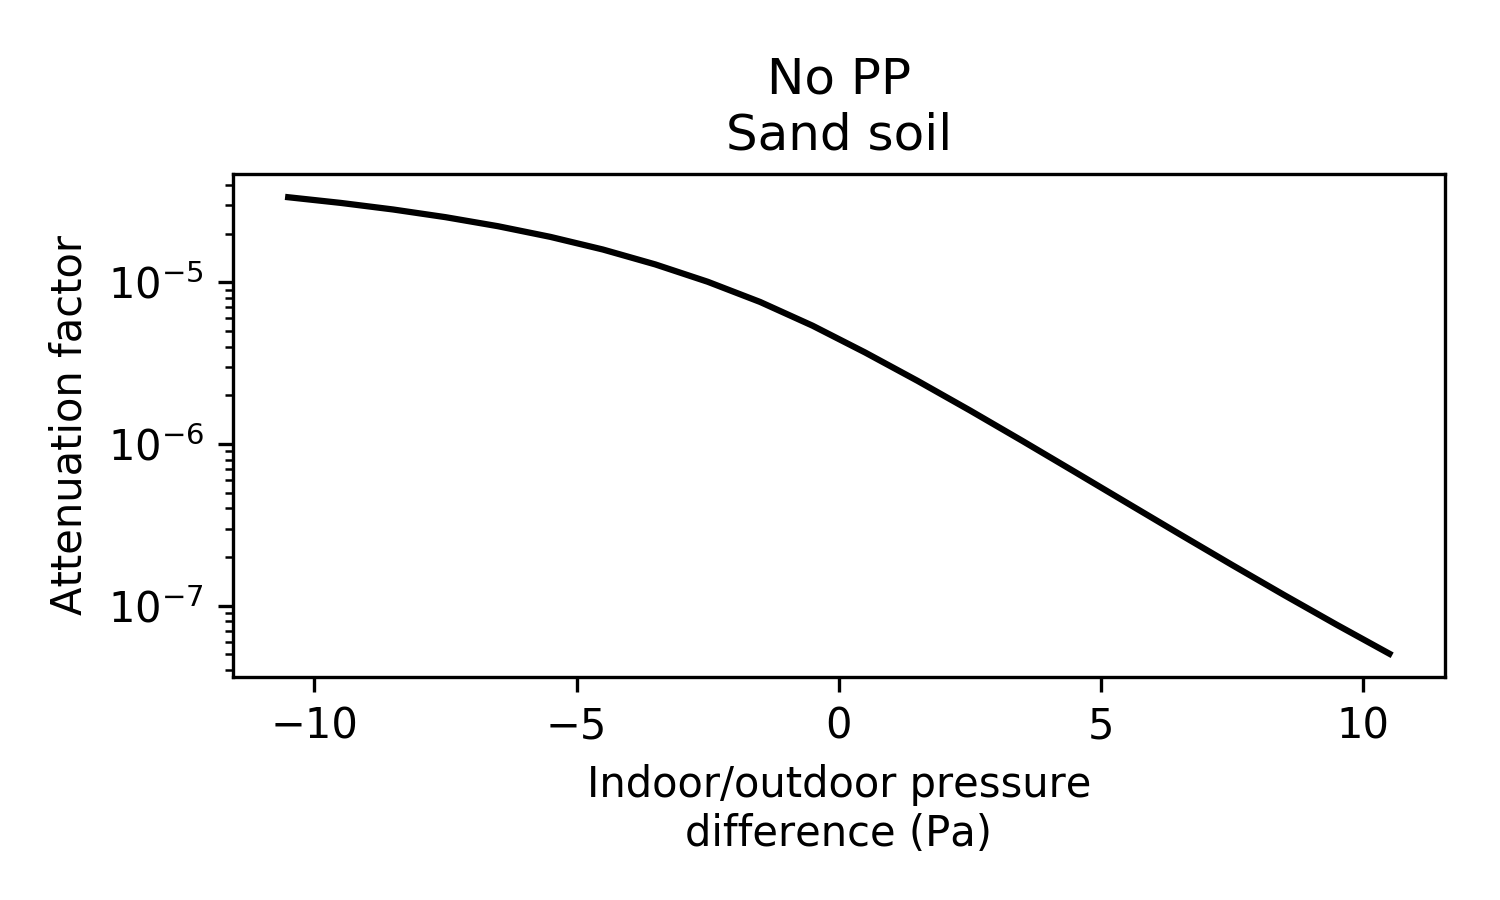
\includegraphics[width=\textwidth]{ss_north_island.png}
  \end{subfigure}
\end{figure}

At the ASU house, after the PP was closed, there was still roughly an order of magnitude variation in IACC, the reasons for which Figure \ref{fig:model_results_sensitivity_analysis} does not address.
Likewise, there was more than two orders of magnitude observed at the North Island site over the indoor-outdoor pressure difference ranges simulated despite there not being a PP present.
Therefore, it is of interest to examine these sites a bit further using the model.

The foundation crack at the ASU house seems by all accounts to be quite small, roughly 180x1 cm and located close to the PP\cite{guo_vapor_2015}.
This crack is smaller than the one assumed in the model used in Figure \ref{fig:model_results_sensitivity_analysis}.
The influence of indoor-outdoor pressure difference is explored for a case in which a smaller crack area is assumed.
We also consider the effects of having a significantly lower air exchange rate, 0.1 vs. the regular 0.5 per hour.

The results of the case shown in Figure \ref{fig:model_results_sensitivity_analysis_2} is shown in Figure \ref{fig:ss_asu}.
Even though there is an increase in $\alpha_\mathrm{gw}$ with increased underpressurization, it is no where near the roughly one order of magnitude recorded at the ASU house after the PP was closed.
So while crack dimensions can clearly influence $\alpha_\mathrm{gw}$, they cannot be used to infer a bigger role for pressure difference in temporal variations in $\alpha_\mathrm{gw}$ or IACC.
The influence of air exchange rate on $\alpha_\mathrm{gw}$ predictions is also shown in Figure \ref{fig:model_results_asu_north_island}.
Clearly, the value of air exchange rate at steady-state conditions will only influence absolute concentrations in the structure.
Ultimately, the reason for the transient variability in IACC during the post-CPM period at the ASU house remains elusive, as a Pearson's r analysis between IACC and various factors do not yield any explanation.

In the case of the North Island site, variations in IACC are clearly not related to the existence of a PP.
The soil underlying the North Island site is more sand-like\cite{hosangadi_high-frequency_2017}.
The significance of this is that sand soil is much more permeable than sandy clay soil, which means that $\alpha_\mathrm{gw}$ will be much more sensitive to changes in indoor-outdoor pressure difference.
Thus, another "normal" VI scenario was run but this time with sand soil instead of sandy clay, the results of which may be seen in Figure \ref{fig:ss_north_island}.
Under these conditions, $\alpha_\mathrm{gw}$ changes significantly with pressurization, spanning roughly two orders of magnitude.
This is consistent with what was observed at North Island, as there the span of IACC values was roughly the same across this range of indoor-outdoor pressure difference values.
This simulation, together with the Pearson $r = -0.64$ for North Island in Figure \ref{fig:kde-asu-nas} suggest that under conditions where the soil around a structure is relatively permeable, indoor-outdoor pressure difference can be a significant driving forces for transient changes in IACC.
Therefore, recording the indoor-outdoor pressure difference at a site (in particular if the soil is permeable) may offer insight into the potential for transient changes in IACC (some good methods for doing this are suggested by \citeauthor{nielsen_remediation_2017-1}\cite{nielsen_remediation_2017-1}).

% Transient part
\subsubsection{Transient Modeling}

Analyzing the impact of a PP using steady-state simulations such as those in Figures \ref{fig:model_results_sensitivity_analysis} and does not revealing about how quickly IACC can change in the presence of a PP.
A transient simulation of a VI scenario that is characterized by a PP has been performed, where only the indoor-outdoor pressure difference was temporally changed.
The pressure difference is changed in a sinusoidal fashion, defined by \eqref{eq:p_transient},
\begin{equation}
  \label{eq:p_transient}
  p_\mathrm{in/out} = 10 \sin{(2 \pi t)} - 0.5
\end{equation}
where $t$ is given in days and $p_\mathrm{in/out}$ is the indoor-outdoor pressure difference in Pa.
Figure \ref{fig:transient_simulation} shows the results of this simulation.

\begin{figure}
  \caption{Transient response of TCE in indoor air (as attenuation factor) and in the surrounding soil \& gravel sub-base for a PP VI scenario subject to sinusoidal indoor-outdoor pressure fluctuations.
  \ref{fig:alpha_response} shows the attenuation factor and indoor-outdoor pressure across time.
  Figures \ref{fig:soil_30_hr} \& \ref{fig:soil_42_hr} show the contaminant concentration (normalized to the contaminant vapor in equilibrium with groundwater) in the surrounding soil \& gravel sub-base at different depths and times.}
  \label{fig:transient_simulation}
  % Transient response figure
  \begin{subfigure}[t]{0.75\textwidth}
    \caption{ }
    \label{fig:alpha_response}
    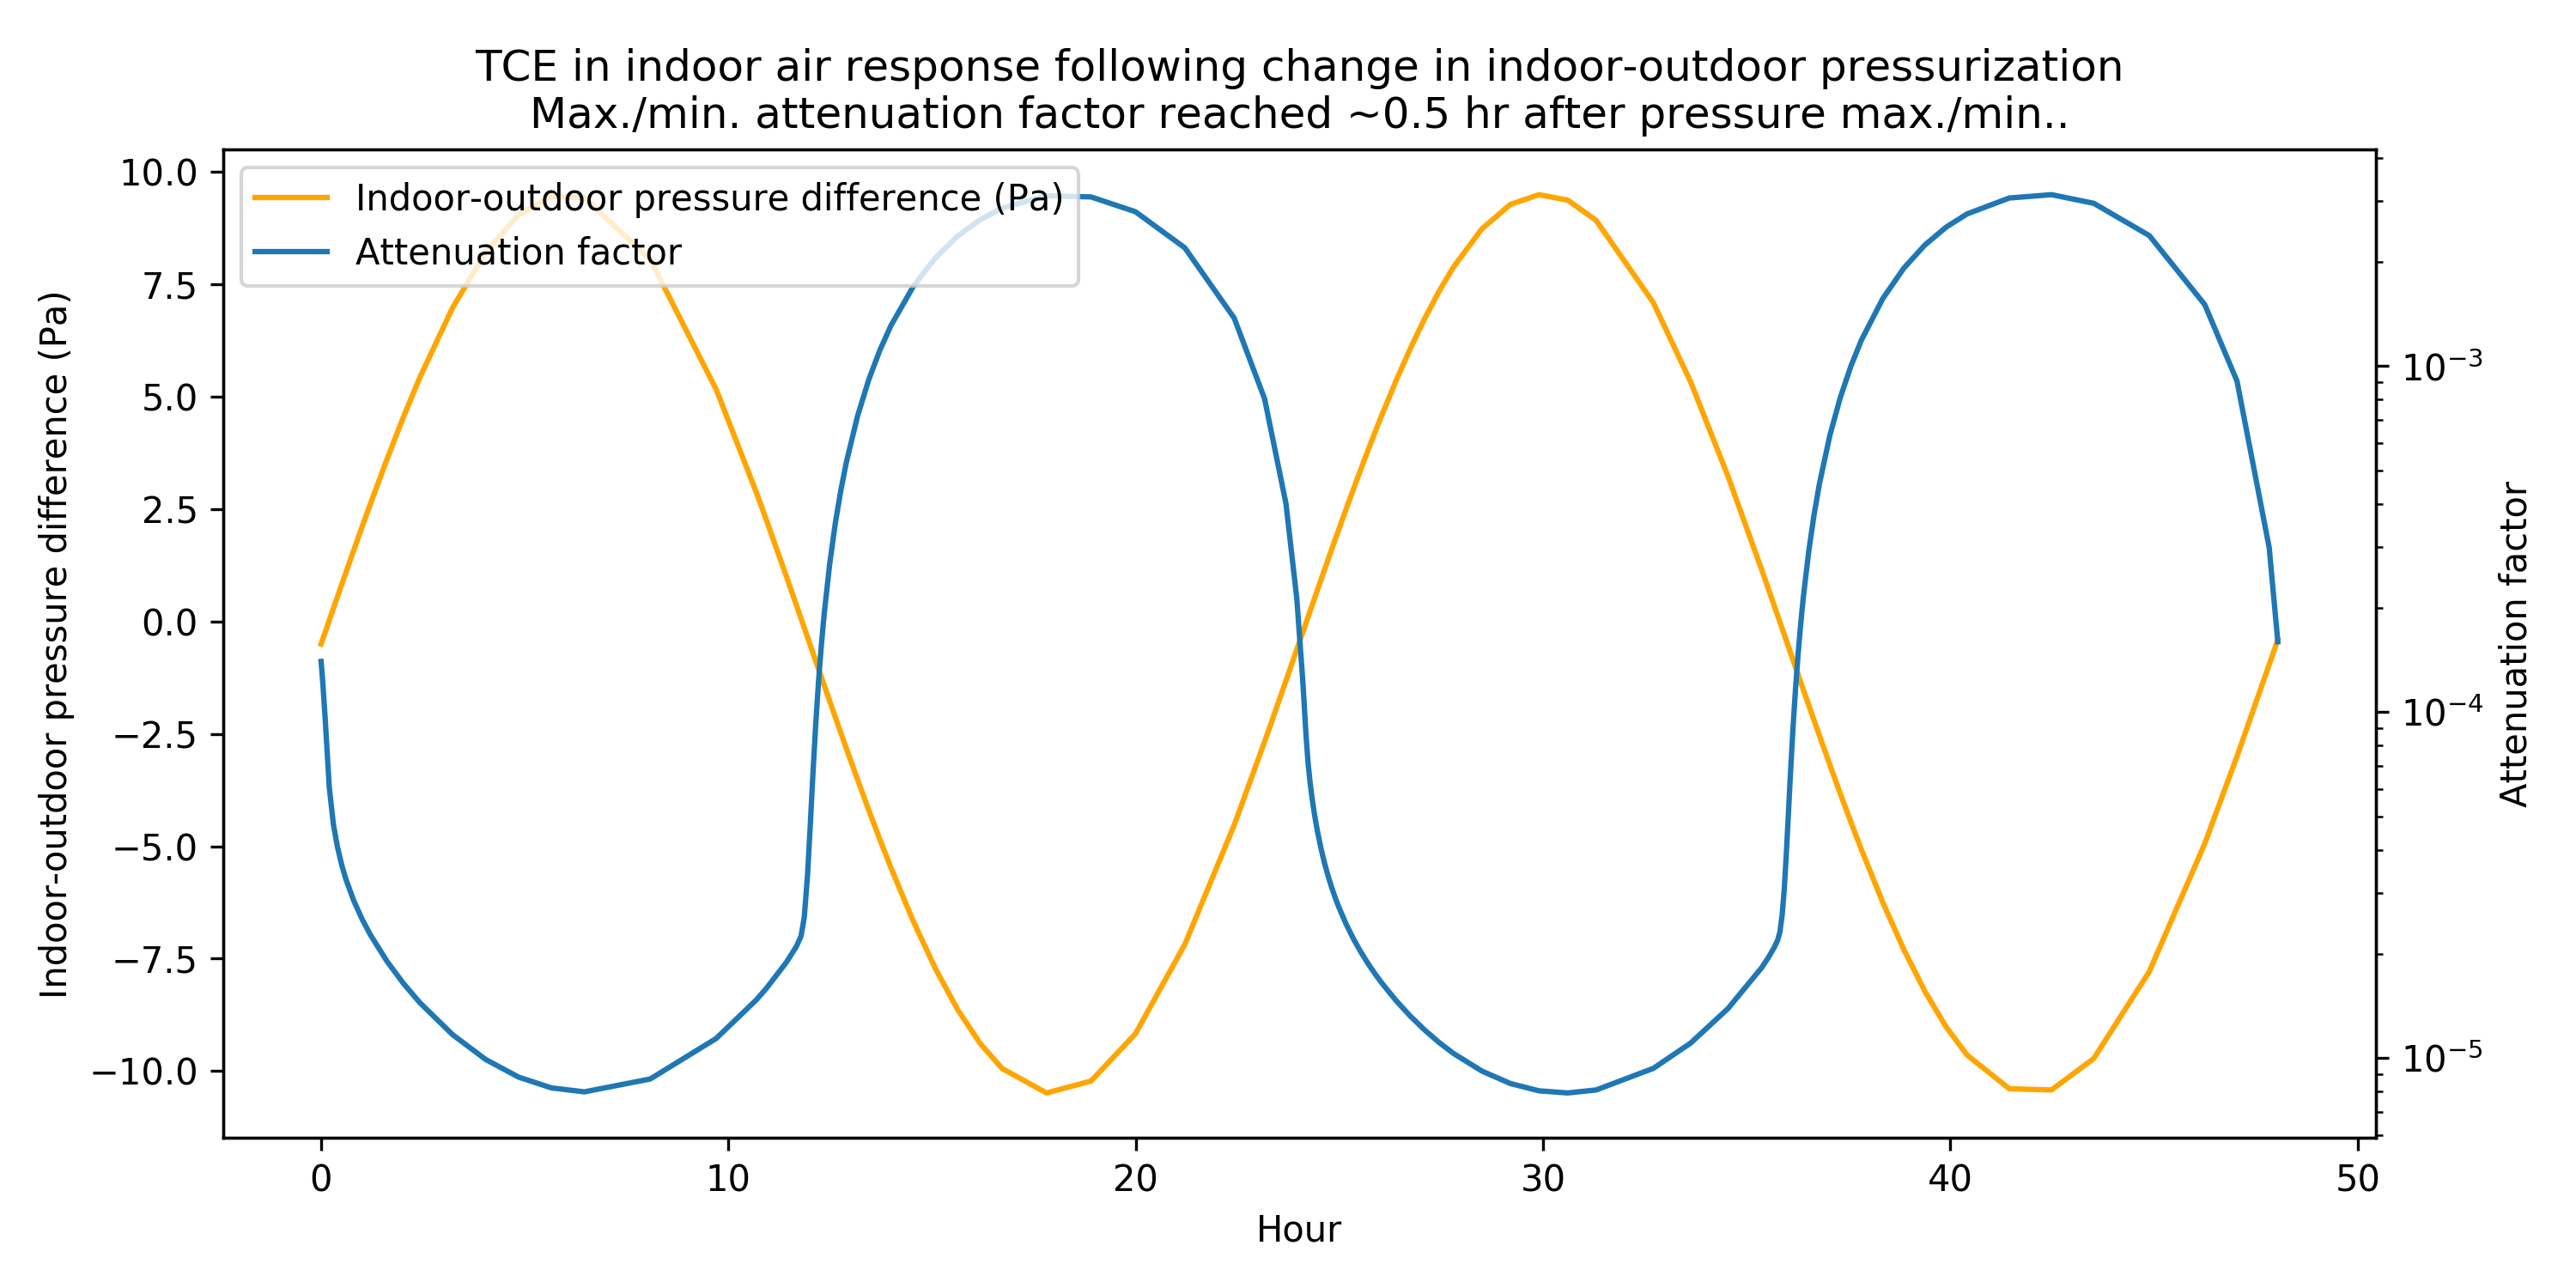
\includegraphics[width=\textwidth]{alpha_transient.png}
  \end{subfigure}
  % Soil t = 30 hr ...
  \begin{subfigure}[c]{0.45\textwidth}
    \caption{t = 30 hr}
    \label{fig:soil_30_hr}
    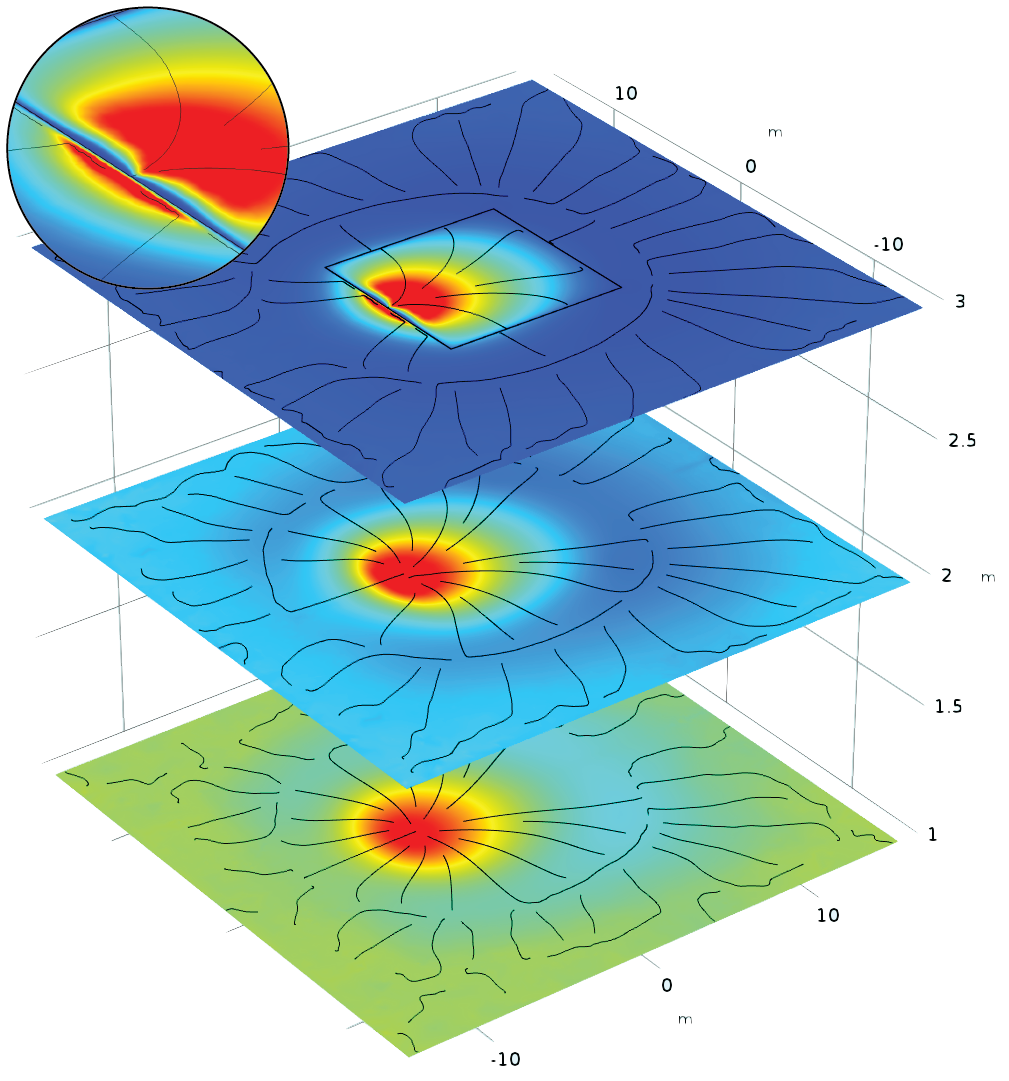
\includegraphics[width=\textwidth]{tri_layer_soil_concs1.png}
  \end{subfigure}
  % Soil t = 42 hr ...
  \begin{subfigure}[c]{0.45\textwidth}
    \caption{t = 42 hr}
    \label{fig:soil_42_hr}
    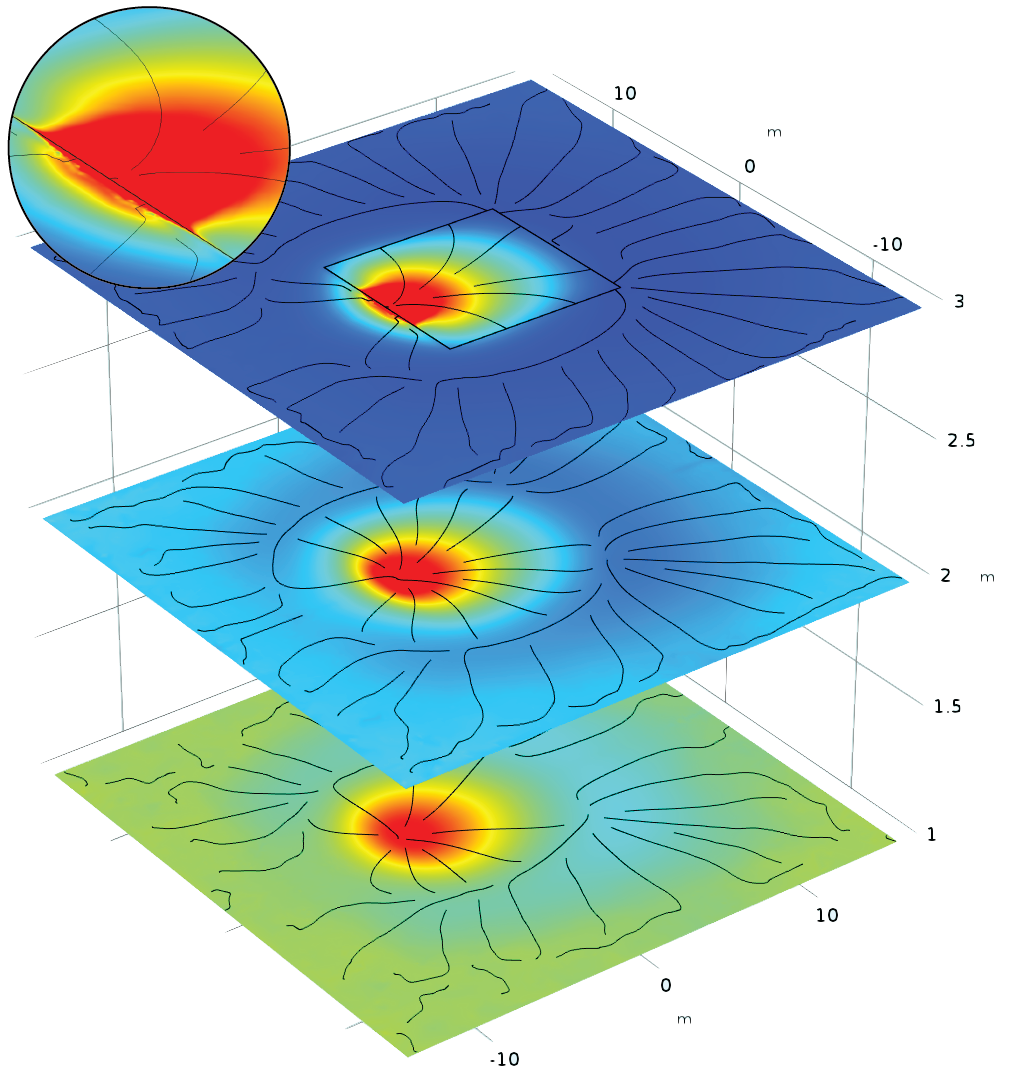
\includegraphics[width=\textwidth]{tri_layer_soil_concs2.png}
  \end{subfigure}
  % Color map
  \begin{subfigure}[c]{0.05\textwidth}
    \phantomcaption{ }
    %\label{fig:cmap}
    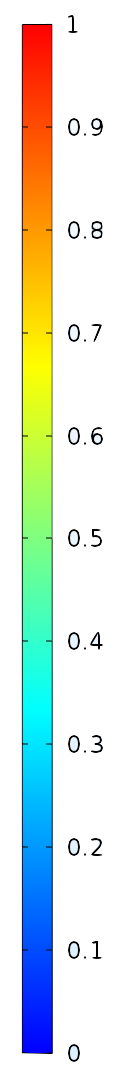
\includegraphics[width=\textwidth]{cmap.png}
  \end{subfigure}
\end{figure}

Figure \ref{fig:alpha_response} shows the IACC response, given as attenuation factor relative to contaminant vapor in equilibrium with groundwater, and the indoor-outdoor pressure difference with time.
What is apparent is that $\alpha_\mathrm{gw}$ closely follows the indoor-outdoor pressure difference, with the max./min. $\alpha_\mathrm{gw}$ being reached roughly 0.5 hours after the indoor-outdoor pressure difference reaches its max./min..
The reader should be aware that the assumption that the indoor air space can be modeled as a CST overestimates how dynamic this process is as a real house probably would not be perfectly mixed on as a short time scale as this.
Regardless, this suggests that VI sites characterized by PPs are highly dynamic and IACC's may change quickly in response to changing indoor-outdoor pressure differences, consistent with what was observed at the ASU house\cite{holton_temporal_2013}.
Again, the dynamics of the indoor-outdoor pressure difference at a VI site can offer insight into the potential for transient behavior of IACC.

Figures \ref{fig:soil_30_hr} and \ref{fig:soil_42_hr} show the contaminant concentration (normalized to the contaminant vapor in equilibrium with groundwater) in the soil and gravel sub-base at three different depths at times of 30 and 42 hr respectively corresponding to roughly the maximum in overpressurization and depressurization respectively.
The top layer is 3 m above groundwater and immediately under the house foundation (indicated by the black square).
The middle and bottom layers are 2 and 1 m above groundwater respectively.
The black streamlines show the contaminant transport flow paths.
The region closest to the PP is expanded in the circular insets.

The impact of the PP on the contaminant vapor concentration in the subsurface is apparent in these figures, as one easily sees how (especially) the gravel sub-base is filled up.
The contaminant vapor concentration is the highest closest to the PP (which is located at the edge of the gravel sub-base) and decreases with increased distance from the PP.
Note that a very small amount of contaminant vapor leaves the gravel sub-base, as the sandy clay has a relatively large resistance to transport compared with gravel.
This makes it difficult to detect the contribution of the PP outside the foundation footprint.
However, this may not always be true, as vapor contaminant from the PP would disperse more easily into more permeable soils.

It should also be noted that the vapor contaminant emanating from the PP in this model is relatively high concentration; the vapor contaminant concentration is equal to that in equilibrium with the groundwater source.
This does not always seem to be the case, as VI sites that have uncovered PPs find that the vapor contaminant emanating from the PP can be lower than that\cite{guo_vapor_2015}.
Therefore, it may be much more difficult than it may appear in Figures \ref{fig:soil_30_hr} and \ref{fig:soil_42_hr} to localize a vapor contaminant hotspot as a way to determining the presence of a PP at a particular VI site.

The insert circles in figures \ref{fig:soil_30_hr} and \ref{fig:soil_42_hr} also show that for the simulated time period, only a small amount of the contaminant enters the structure (as evident by the blue low concentration zone around the perimeter), yet a very large increase in $\alpha_\mathrm{gw}$ occurs.
The concentration in the rest of the sub-base is unchanged.
This suggests that once a PP has deposited contaminant underneath a structure, it may persist for a long time period, as pointed out by \citeauthor{guo_vapor_2015}\cite{guo_vapor_2015}.

\end{comment}

\begin{acknowledgement}
This project was supported by grant ES-201502 from the Strategic Environmental Research and Development Program and Environmental Security Technology Certification Program (SERDP-ESTCP).
\end{acknowledgement}

\begin{table}[htb!]
  \caption{Abbreviations \& symbols}
  \begin{tabular}{l l}
  \toprule
  \textbf{Abbreviation or symbol}     & \textbf{Explanation} \\
  % General abbreviations
  VI                                  & Vapor intrusion \\
  PP                                  & Preferential pathway \\
  $L_\mathrm{slab}$                   & Thickness of the foundation concrete slab \\
  % Richard's equation
  $p$                                 & Pressure \\
  % Unsteady-cstr
  $u$                                 & TCE in indoor air concentration \\
  $c$                                 & TCE in soil gas concentration \\
  % Diffusion stuff
  $D_\mathrm{air}$                    & Diffusion of TCE in air \\
  $D_\mathrm{water}$                  & Diffusion of TCE in water \\
  $D_\mathrm{eff}$                    & Effective Diffusion of TCE in soil \\
  $K_H$                               & Henry's Law constant \\
  % van Genuchten stuff
  $\theta_g, \theta_w\;\&\;\theta_s$  & Vapor, water filled \& saturated soil porosity \\
  $\theta_r$                          & Residual moisture porosity \\
  $\alpha,\; l,\; n\;\&\; m$          & van Genuchten parameters \\
  $\mathrm{Se}$                       & Soil moisture saturation \\
  $k_r$                               & Relative permeability \\
  $\alpha_\mathrm{gw}$                & Attenuation factor \\
  \bottomrule
  \end{tabular}
\end{table}

\bibliography{library}

\end{document}
